\documentclass{aomart}

\usepackage[T1]{fontenc}
\usepackage[nopatch=footnote]{microtype}
\usepackage{amssymb,mathtools}
\usepackage{bm}
\usepackage{aliascnt}
\usepackage{enumitem}
\usepackage{graphicx}
\usepackage{booktabs}
\usepackage{array}
\usepackage{longtable}
\usepackage[nameinlink,noabbrev]{cleveref}

\allowdisplaybreaks
\hyphenpenalty=10000
\exhyphenpenalty=10000
\tolerance=2500
\emergencystretch=4em

\makeatletter
\def\@setsubjects{%
  \let\@subjects\@empty
  \ifx\@primarysubjects\@empty\else
    \edef\@subjects{Primary:~\@primarysubjects}%
  \fi
  \ifx\@secondarysubjects\@empty\else
    \ifx\@primarysubjects\@empty
      \edef\@subjects{Secondary:~\@secondarysubjects}%
    \else
      \edef\@subjects{\@subjects, Secondary:~\@secondarysubjects}%
    \fi
  \fi
  \ifpdf
    \hypersetup{pdfsubject=\@subjects}%
  \fi
  \if@aom@oldkeywords\else
    \@footnotetext{AMS Classification:~\@subjects.}%
  \fi
}
\makeatother

\setlist[enumerate]{topsep=4pt,itemsep=2pt}
\setlist[itemize]{topsep=4pt,itemsep=2pt}

\newtheorem{theorem}{Theorem}[section]
\newaliascnt{proposition}{theorem}
\newtheorem{proposition}[proposition]{Proposition}
\aliascntresetthe{proposition}
\newaliascnt{lemma}{theorem}
\newtheorem{lemma}[lemma]{Lemma}
\aliascntresetthe{lemma}
\newaliascnt{corollary}{theorem}
\newtheorem{corollary}[corollary]{Corollary}
\aliascntresetthe{corollary}
\theoremstyle{definition}
\newaliascnt{definition}{theorem}
\newtheorem{definition}[definition]{Definition}
\aliascntresetthe{definition}
\newaliascnt{example}{theorem}
\newtheorem{example}[example]{Example}
\aliascntresetthe{example}
\newaliascnt{standardfact}{theorem}
\newtheorem{standardfact}[standardfact]{Standard Fact}
\aliascntresetthe{standardfact}
\theoremstyle{remark}
\newaliascnt{remark}{theorem}
\newtheorem{remark}[remark]{Remark}
\aliascntresetthe{remark}

\crefname{theorem}{theorem}{theorems}
\crefname{proposition}{proposition}{propositions}
\crefname{lemma}{lemma}{lemmas}
\crefname{corollary}{corollary}{corollaries}
\crefname{definition}{definition}{definitions}
\crefname{example}{example}{examples}
\crefname{standardfact}{standard fact}{standard facts}
\crefname{remark}{remark}{remarks}

\newcommand{\CC}{\mathbb C}
\newcommand{\RR}{\mathbb R}
\newcommand{\NN}{\mathbb N}
\newcommand{\Acal}{\mathcal A}
\newcommand{\Bcal}{\mathcal B}
\newcommand{\Ccal}{\mathcal C}
\newcommand{\Dcal}{\mathcal D}
\newcommand{\Ecal}{\mathcal E}
\newcommand{\Fcal}{\mathcal F}
\newcommand{\Gcal}{\mathcal G}
\newcommand{\Hcal}{\mathcal H}
\newcommand{\Kcal}{\mathcal K}
\newcommand{\Lcal}{\mathcal L}
\newcommand{\Mcal}{\mathcal M}
\newcommand{\Pcal}{\mathcal P}
\newcommand{\Qcal}{\mathcal Q}
\newcommand{\Rcal}{\mathcal R}
\newcommand{\Scal}{\mathcal S}
\newcommand{\Tcal}{\mathcal T}
\newcommand{\Ucal}{\mathcal U}
\newcommand{\Vcal}{\mathcal V}
\newcommand{\End}{\operatorname{End}}
\newcommand{\Ran}{\operatorname{Ran}}
\newcommand{\Ker}{\operatorname{Ker}}
\newcommand{\Spec}{\operatorname{Spec}}
\newcommand{\Tr}{\operatorname{Tr}}
\newcommand{\tr}{\operatorname{tr}}
\newcommand{\rank}{\operatorname{rank}}
\newcommand{\diag}{\operatorname{diag}}
\newcommand{\cond}{\operatorname{cond}}
\newcommand{\supp}{\operatorname{supp}}
\newcommand{\flop}{\operatorname{flop}}
\newcommand{\bytes}{\operatorname{bytes}}
\newcommand{\cost}{\operatorname{cost}}
\newcommand{\err}{\operatorname{err}}
\newcommand{\e}{\mathrm e}
\newcommand{\ii}{\mathrm i}
\newcommand{\id}{\mathrm{id}}
\newcommand{\norm}[1]{\left\lVert#1\right\rVert}
\newcommand{\abs}[1]{\left\lvert#1\right\rvert}
\newcommand{\ip}[2]{\left\langle#1,#2\right\rangle}
\newcommand{\one}{\bm 1}
\newcommand{\eps}{\varepsilon}
\newcommand{\IR}{\mathsf{IR}}
\newcommand{\Ical}{\mathcal I}
\newcommand{\dist}{\operatorname{dist}}
\newcommand{\DP}{\mathsf{DP}}

\graphicspath{{figures/}}

\title[Packet operator algorithms]{Packet Operator Algorithms, Exact Compilation, and GPU Realization}
\author[Komorebi P.]{Komorebi P.}
\subject{primary}{msc2020}{65F30}
\subject{secondary}{msc2020}{65F50}
\subject{secondary}{msc2020}{65Y05}
\subject{secondary}{msc2020}{68W10}
\subject{secondary}{msc2020}{68W40}
\keyword{structured matrix}
\keyword{low rank update}
\keyword{dynamic programming}
\keyword{mixed precision}
\keyword{GPU computation}
\keyword{benchmark contract}
\copyrightnote{}
\doinumber{}

\pdfstringdefDisableCommands{\let\unskip\relax}
\hypersetup{
  pdftitle={Packet Operator Algorithms, Exact Compilation, and GPU Realization},
  pdfauthor={Komorebi P.},
  pdfsubject={Packet operator representations, exact tree compilation, low rank algebra, mixed precision, scheduling, and measured GPU realization}
}

\begin{document}
\begin{abstract}
A packet operator is a linear map written between the members of a finite direct sum. We study the resulting computational representation before choosing a processor or kernel. Exact formulas are given for block sparse application, block diagonal plus low rank algebra, Woodbury inversion, support propagation, block preconditioning, and packetwise perturbation. Products of low rank corrections admit optimal recompression through a small singular value problem, with explicit error propagation through a product chain. A rooted candidate decomposition supports an exact compiler when representation cost and error are additive. Dynamic programming gives the optimal Lagrangian pruning, an exact quantized error budget algorithm, and a local update rule. Discrete precision assignment becomes a multiple choice budget problem. Arithmetic, storage, data movement, launch count, discovery, transfer, and materialization are kept as separate costs. A sanitized corpus of 154 recorded CPU and GPU measurements illustrates regular packet gains, precision frontiers, crossover behavior, and retained negative controls. The largest matched structured result is a factor of 14.89 against a device resident dense GPU calculation. The paper proves finite algebraic and optimization statements. Hardware measurements remain specific to their recorded environment, and no generic dense matrix exponent or universal discovery algorithm is claimed.
\end{abstract}
\maketitle
\thispagestyle{plain}

\section{Introduction}\label{sec:introduction}

A matrix can look dense while its action is not. Independent diagonal blocks, sparse transfers, low rank couplings, tensor factors, and transform coordinates can remove most of the arithmetic and storage before a kernel is launched. The gain is mathematical first. A device can exploit only the structure that the representation exposes.

This article begins with a finite direct sum
\[
X=\bigoplus_{\alpha\in I}X_\alpha
\]
and a complete family of coordinate projectors
\[
P_\alpha P_\beta=\delta_{\alpha\beta}P_\alpha,
\qquad
\sum_{\alpha\in I}P_\alpha=I.
\]
An operator has packet blocks
\[
A_{\beta\alpha}=P_\beta AP_\alpha.
\]
The active addresses form a directed graph. Block dimensions, block types, approximation tolerances, and output requirements turn this graph into a computational intermediate representation.

The underlying linear algebra is classical. Direct and iterative methods are treated in \cite{GolubVanLoan2013,Saad2003,Davis2006}. Low rank approximation and updates are governed by singular value decomposition and the Sherman Morrison Woodbury identity \cite{EckartYoung1936,Mirsky1960,Hager1989,BunchNielsen1978}. Floating point analysis follows the standard model in \cite{Higham2002,IEEE7542019}. Randomized discovery of low rank structure is developed in \cite{HalkoMartinssonTropp2011,MartinssonTropp2020}. Communication and attainable performance are shaped by data movement and arithmetic intensity \cite{HongKung1981,WilliamsWatermanPatterson2009,BallardDemmelHoltzSchwartz2011,FrigoLeisersonProkopRamachandran1999}.

The first task is semantic. A compressed representation must specify the operator that it denotes. It must also specify what an algorithm returns. A product represented by block and low rank factors is not the same output as an explicit matrix. A timing comparison is valid only after the output contract and timing scope agree.

The second task is algebraic. Block diagonal plus low rank operators are closed under multiplication before recompression. Their unrecompressed rank grows additively. Woodbury inversion reduces a large inverse to packet solves and one small dense inverse. The low rank factors can then be recompressed by orthogonalizing them and taking the singular value decomposition of a small core. This produces the best truncated approximation in spectral and Frobenius norm.

The third task is combinatorial. Sparse transfer graphs predict possible support under powers, polynomials, and Schur elimination. A directed acyclic graph gives a finite path expansion. A block triangular solve can be scheduled by topological level. Graph regularity matters because equal shapes can be batched, while irregular edges require indexing and accumulation.

The fourth task is numerical. Packet perturbations can be certified by their block sensitivities. A continuous model assigns tolerances through a convex calculation. Upper bounds on available tolerances produce a clipped allocation. A finite set of data types gives a multiple choice budget problem that can be solved exactly after the errors are quantized.

The central computational result concerns compilation. Suppose a finite rooted tree records candidate refinements. Each node may be kept as one representation or split into its children. If cost and error are additive across the selected leaves, the optimal pruning is found exactly by dynamic programming. A quantized error budget has a second exact dynamic program. The decision is stable when the score gap exceeds the perturbation in the local models. A change inside one subtree requires recomputation only along the ancestor chain. These results prove a restricted packet compiler. They do not solve unrestricted discovery or arbitrary device scheduling.

The measured part uses a sanitized corpus collected on one recorded CPU and one NVIDIA GeForce RTX 3070 Ti Laptop GPU. The corpus contains 154 measured rows from sixteen suites. Regular equal block operators and block diagonal plus low rank operators show large gains. Recursive HODLR, Strassen multiplication, iterative refinement, a small Walsh Hadamard transform, and an attempted two stream overlap provide negative controls. These rows are retained because structure does not guarantee speed.

The article separates four sources of gain:
\[
\text{representation},
\qquad
\text{device},
\qquad
\text{kernel},
\qquad
\text{amortization}.
\]
A single speedup number can mix all four. The benchmark protocol therefore records case identity, output contract, timing scope, source precision, correctness reference, discovery time, compilation time, and reuse count.

\begin{figure}[t]
\centering
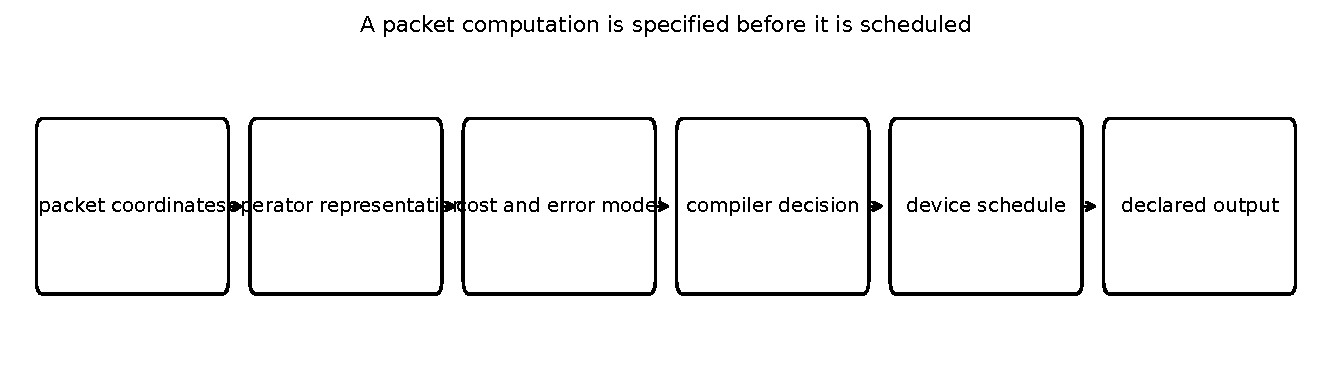
\includegraphics[width=\textwidth]{01_packet_compilation_architecture.pdf}
\caption{The representation and the output contract are fixed before the device schedule is chosen.}
\label{fig:architecture}
\end{figure}

The mathematical statements are finite. The empirical statements apply only to the recorded environment and generated cases. The article does not claim a new generic matrix multiplication exponent. Fast matrix multiplication and its stability form a separate theory \cite{Strassen1969,DemmelHoltzSchwartz2007}. It also does not claim that every structured matrix has a profitable GPU realization.

\section{Packet operator representations}\label{sec:ir}

\subsection{Exact semantics}

\begin{definition}[Packet layout]\label{def:packet_layout}
A packet layout is a finite family of finite dimensional Hilbert spaces
\[
\Pcal=(X_\alpha)_{\alpha\in I}
\]
with direct sum
\[
X=\bigoplus_{\alpha\in I}X_\alpha.
\]
Write
\[
n_\alpha=\dim X_\alpha,
\qquad
n=\sum_{\alpha\in I}n_\alpha.
\]
The coordinate projector onto \(X_\alpha\) is denoted by \(P_\alpha\).
\end{definition}

\begin{definition}[Packet operator representation]\label{def:packet_ir}
A finite packet operator representation consists of
\[
\IR=(\Pcal,E,(B_{\beta\alpha})_{(\beta,\alpha)\in E}),
\]
where
\[
E\subseteq I\times I
\]
and
\[
B_{\beta\alpha}:X_\alpha\longrightarrow X_\beta.
\]
Its evaluation is
\[
\operatorname{eval}(\IR)
=
\sum_{(\beta,\alpha)\in E}
\iota_\beta B_{\beta\alpha}P_\alpha,
\]
where \(\iota_\beta:X_\beta\to X\) is the coordinate inclusion.
\end{definition}

\begin{theorem}[Exact evaluation]\label{thm:exact_evaluation}
Let \(A\in\End(X)\). Set
\[
B_{\beta\alpha}=P_\beta AP_\alpha
\]
and let \(E\) contain exactly the nonzero blocks. Then
\[
\boxed{
A=
\sum_{(\beta,\alpha)\in E}
P_\beta AP_\alpha.
}
\]
For every matrix of right hand sides \(Z\),
\[
AZ
=
\sum_{(\beta,\alpha)\in E}
B_{\beta\alpha}P_\alpha Z.
\]
\end{theorem}

\begin{proof}
Insert the identity on both sides of \(A\):
\[
A
=
\left(\sum_\beta P_\beta\right)
A
\left(\sum_\alpha P_\alpha\right)
=
\sum_{\alpha,\beta}P_\beta AP_\alpha.
\]
The zero blocks can be removed. Applying the identity to \(Z\) gives the second formula.
\end{proof}

\begin{definition}[Support graph]\label{def:support_graph}
The support graph \(G_A\) has vertex set \(I\). It has a directed edge
\[
\alpha\longrightarrow\beta
\]
when \(P_\beta AP_\alpha\neq0\).
\end{definition}

\begin{figure}[t]
\centering
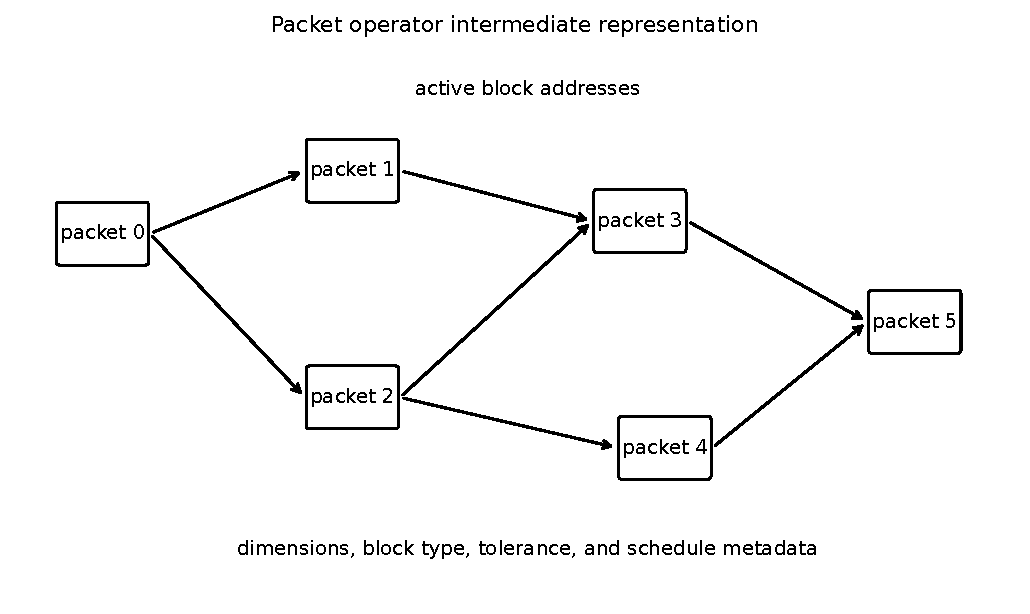
\includegraphics[width=.88\textwidth]{02_packet_ir_graph.pdf}
\caption{A packet intermediate representation stores active block addresses together with dimensions, block types, tolerances, and scheduling metadata.}
\label{fig:packet_ir}
\end{figure}

\begin{theorem}[Block composition]\label{thm:block_composition}
Let \(A,B\in\End(X)\). Then
\[
\boxed{
(AB)_{\gamma\alpha}
=
\sum_{\beta\in I}
A_{\gamma\beta}B_{\beta\alpha}.
}
\]
Consequently,
\[
\supp(AB)
\subseteq
\supp(A)\circ\supp(B),
\]
where relational composition is defined by
\[
(\gamma,\alpha)\in E\circ F
\]
when some \(\beta\) satisfies
\[
(\gamma,\beta)\in E,
\qquad
(\beta,\alpha)\in F.
\]
\end{theorem}

\begin{proof}
Insert the packet identity between \(A\) and \(B\):
\[
P_\gamma ABP_\alpha
=
\sum_\beta
P_\gamma AP_\beta BP_\alpha.
\]
A summand can be nonzero only when both block addresses are active.
\end{proof}

\begin{corollary}[Adjoint and tensor semantics]\label{cor:adjoint_tensor}
The adjoint representation has blocks
\[
(A^*)_{\alpha\beta}=A_{\beta\alpha}^*.
\]
If \(A\) and \(B\) are packet resolved on \(X\) and \(Y\), then
\[
(A\otimes B)_{(\beta,\delta),(\alpha,\gamma)}
=
A_{\beta\alpha}\otimes B_{\delta\gamma}.
\]
\end{corollary}

\begin{proof}
Both identities follow by inserting the corresponding coordinate projectors and using
\[
(P_\beta AP_\alpha)^*=P_\alpha A^*P_\beta.
\]
The tensor identity follows from
\[
(P_\beta\otimes Q_\delta)
(A\otimes B)
(P_\alpha\otimes Q_\gamma)
=
A_{\beta\alpha}\otimes B_{\delta\gamma}.
\]
\end{proof}

\subsection{Output contracts}

\begin{definition}[Output contract]\label{def:output_contract}
An output contract specifies the mathematical object returned by an algorithm. The contract may require an explicit vector, an explicit matrix, block factors, low rank factors, spectral factors, or an implicit operator with a declared application rule.
\end{definition}

\begin{definition}[Timing scope]\label{def:timing_scope}
A timing scope states which costs are included. Possible costs include structure discovery, compilation, host transfer, device transfer, kernel execution, graph capture, graph replay, factor reconstruction, and explicit materialization.
\end{definition}

\begin{proposition}[Contract conversion]\label{prop:contract_conversion}
Suppose one algorithm returns a compressed representation \(R\) and another returns an explicit object \(Y\). A direct timing comparison is valid only if
\[
\operatorname{decode}(R)=Y
\]
and the time required by \(\operatorname{decode}\) is included, or if the downstream task consumes \(R\) directly.
\end{proposition}

\begin{proof}
Without decoding, the two procedures return different mathematical objects. A timing ratio between different outputs does not compare implementations of the same map. Including the decoding cost gives two procedures with the same output. If the next operation consumes \(R\), decoding is not part of the declared computation.
\end{proof}

\begin{remark}\label{rem:semantic_boundary}
A compressed product and an explicit matrix product may both be exact. They still have different contracts. This distinction becomes decisive when materialization costs \(n^2\) entries.
\end{remark}

\section{Arithmetic, storage, and data movement}\label{sec:cost}

We count one scalar multiplication and one scalar addition as two modeled floating point operations. These counts describe a representation. They do not predict wall time without a memory and launch model.

\begin{theorem}[Dense and packet application counts]\label{thm:packet_counts}
A dense \(n\) by \(n\) matrix applied to \(q\) right hand sides has modeled cost
\[
\boxed{
\flop_{\rm dense}=2n^2q.
}
\]
A packet representation with active edge set \(E\) has modeled cost
\[
\boxed{
\flop_{\rm packet}
=
2q
\sum_{(\beta,\alpha)\in E}
n_\beta n_\alpha.
}
\]
It stores
\[
\boxed{
M_{\rm packet}
=
\sum_{(\beta,\alpha)\in E}
n_\beta n_\alpha
}
\]
scalar entries.
\end{theorem}

\begin{proof}
The active block \(B_{\beta\alpha}\) is an \(n_\beta\) by \(n_\alpha\) matrix. Applying it to an \(n_\alpha\) by \(q\) input costs \(2n_\beta n_\alpha q\) modeled operations and stores \(n_\beta n_\alpha\) scalars. Summation over the active addresses gives both formulas.
\end{proof}

\begin{corollary}[Equal diagonal packets]\label{cor:equal_blocks}
Suppose \(n\) is divided into equal diagonal packets of width \(b\). Then
\[
\flop_{\rm block}=2qnb,
\qquad
M_{\rm block}=nb.
\]
The dense to block reduction factor is
\[
\boxed{
\frac{n}{b}.
}
\]
\end{corollary}

\begin{proof}
There are \(n/b\) active diagonal blocks. Each contains \(b^2\) entries.
\end{proof}

\begin{definition}[Block diagonal plus low rank operator]\label{def:bdlr}
A block diagonal plus low rank operator has the form
\[
A=D+UV^*,
\]
where
\[
D=\bigoplus_{\alpha\in I}D_\alpha,
\qquad
U,V\in\CC^{n\times r}.
\]
The abbreviation BDLR will be used below.
\end{definition}

\begin{theorem}[BDLR application and storage]\label{thm:bdlr_counts}
For \(q\) right hand sides,
\[
AZ=DZ+U(V^*Z)
\]
has modeled cost
\[
\boxed{
2q
\left(
\sum_\alpha n_\alpha^2+2nr
\right).
}
\]
The representation stores
\[
\boxed{
\sum_\alpha n_\alpha^2+2nr
}
\]
scalars. For equal packets of width \(b\), both ideal dense reduction factors equal
\[
\boxed{
\frac{n}{b+2r}.
}
\]
\end{theorem}

\begin{proof}
The block diagonal product costs
\[
2q\sum_\alpha n_\alpha^2.
\]
The products \(V^*Z\) and \(U(V^*Z)\) cost \(2nrq\) each. Storage consists of the diagonal blocks and the two low rank factors. For equal packets,
\[
\sum_\alpha n_\alpha^2=nb.
\]
\end{proof}

\begin{figure}[t]
\centering
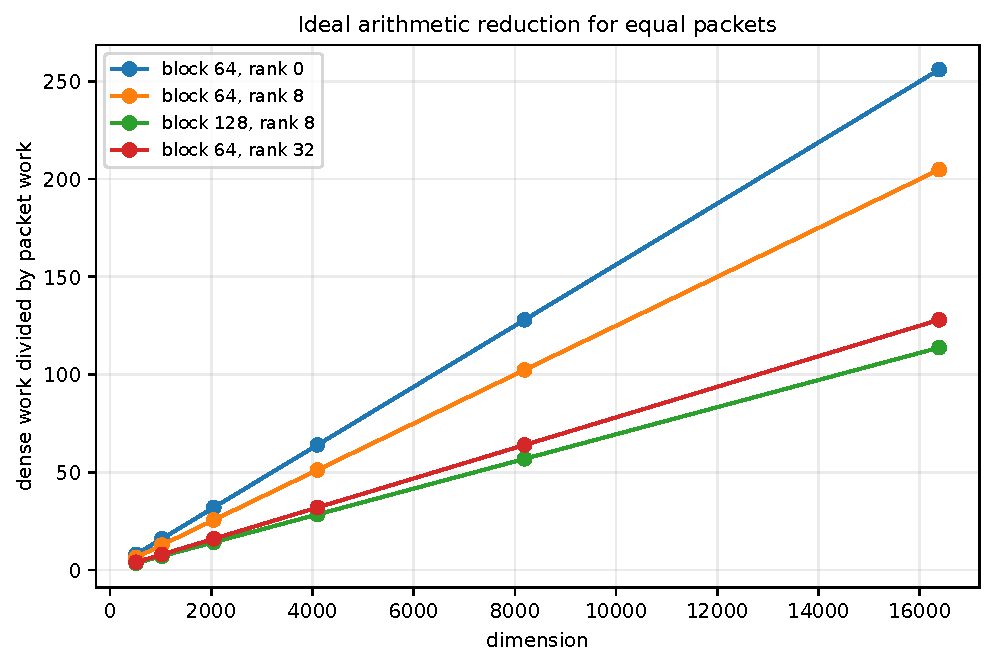
\includegraphics[width=.76\textwidth]{03_ideal_arithmetic_reduction.pdf}
\caption{The ideal reduction grows with dimension only when packet width and transfer rank remain controlled.}
\label{fig:ideal_reduction}
\end{figure}

\begin{definition}[One pass streaming model]\label{def:streaming_model}
Fix a scalar size \(s\) bytes. For every active block, the one pass streaming model reads the block once, reads its source packet once, and reads and writes its target packet once. It does not assume cache reuse across edges.
\end{definition}

\begin{proposition}[Streaming byte count]\label{prop:streaming_bytes}
Under \cref{def:streaming_model}, applying a packet operator to \(q\) right hand sides moves
\[
\boxed{
B_{\rm stream}
=
s
\sum_{(\beta,\alpha)\in E}
\left(
 n_\beta n_\alpha
 +n_\alpha q
 +2n_\beta q
\right)
}
\]
bytes.
\end{proposition}

\begin{proof}
The three terms count the matrix block, the source values, and the read plus write traffic for the target accumulation. The model counts these quantities independently for every active edge.
\end{proof}

\begin{definition}[Arithmetic intensity]\label{def:intensity}
The modeled arithmetic intensity is
\[
\Ical
=
\frac{\flop}{\bytes}.
\]
\end{definition}

\begin{theorem}[Roofline lower bound]\label{thm:roofline}
Suppose a device sustains at most \(P\) modeled operations per second and at most \(W\) bytes per second. A computation that requires \(F\) operations and \(B\) bytes satisfies
\[
\boxed{
T\geq
\max\left\{
\frac{F}{P},
\frac{B}{W}
\right\}.
}
\]
Equivalently, its work rate is at most
\[
\min\{P,W\Ical\}.
\]
\end{theorem}

\begin{proof}
The operation capacity gives \(T\geq F/P\). The bandwidth capacity gives \(T\geq B/W\). Both restrictions hold at once.
\end{proof}

The roofline model is a guide rather than an exact execution law \cite{WilliamsWatermanPatterson2009}. Packet structure changes both \(F\) and \(B\). An irregular representation may remove arithmetic while lowering intensity enough to become bandwidth or launch limited.

\begin{figure}[t]
\centering
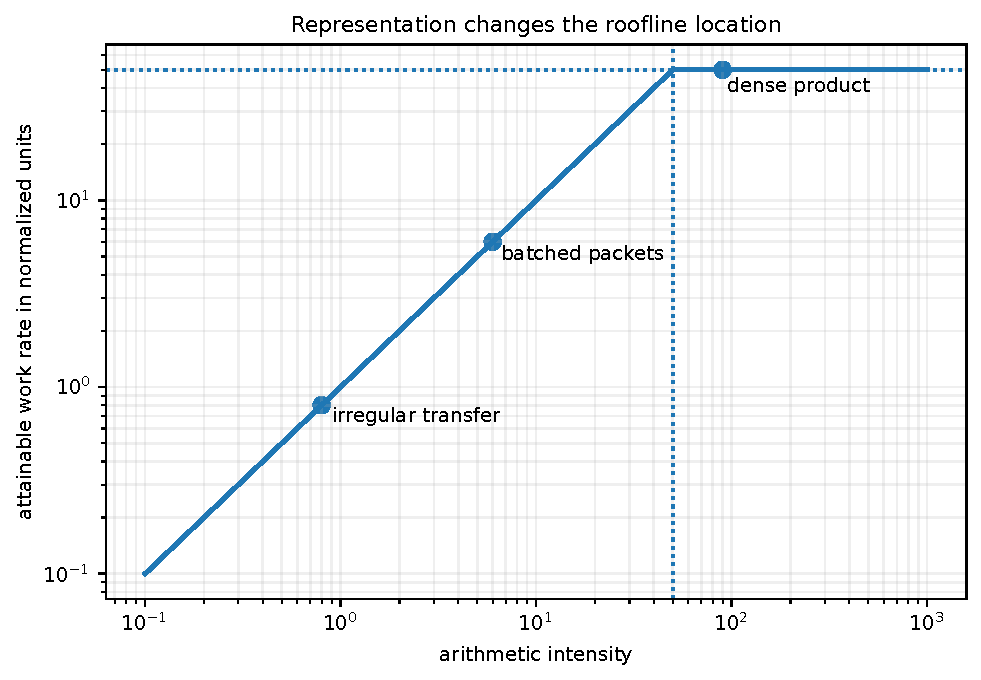
\includegraphics[width=.76\textwidth]{04_roofline_schematic.pdf}
\caption{A representation can move the same mathematical problem between memory limited and compute limited regimes.}
\label{fig:roofline}
\end{figure}

\begin{corollary}[Capacity threshold]\label{cor:capacity}
Let a device have available memory \(M\) bytes and scalar size \(s\). The matrix representation alone can fit only when
\[
n\leq\sqrt{M/s}.
\]
The equal packet BDLR representation alone fits when
\[
n(b+2r)s\leq M.
\]
\end{corollary}

\begin{proof}
Substitute the dense and BDLR storage counts into the capacity inequality.
\end{proof}

\begin{proposition}[Materialization cost]\label{prop:materialization_cost}
Materializing \(D+UV^*\) as an explicit matrix requires storage for \(n^2\) scalars and modeled arithmetic
\[
2n^2r+O(n^2)
\]
when the low rank correction is formed by dense multiplication.
\end{proposition}

\begin{proof}
The product \(UV^*\) multiplies an \(n\) by \(r\) matrix by an \(r\) by \(n\) matrix. Adding the diagonal part changes only the lower order term.
\end{proof}

\section{Structured packet primitives}\label{sec:primitives}

The packet representation can store different exact local operator types. This section records the finite formulas used by several measured suites. The results concern representation and arithmetic. They do not assert that one implementation is fastest at every size.

\begin{proposition}[Equal block banded count]\label{prop:block_banded_count}
Let \(p=n/b\) equal packets have width \(b\). Suppose a block is active precisely when
\[
\abs{i-j}\leq w,
\qquad
0\leq w\leq p-1.
\]
The number of active blocks is
\[
\boxed{
N_{p,w}
=
p(2w+1)-w(w+1).
}
\]
For \(q\) right hand sides, the modeled application cost and scalar storage are
\[
\boxed{
2qb^2N_{p,w}
\quad\text{and}\quad
b^2N_{p,w}.
}
\]
\end{proposition}

\begin{proof}
The diagonal contributes \(p\) blocks. At offset \(k\), where \(1\leq k\leq w\), the upper and lower block diagonals contribute \(2(p-k)\) blocks. Therefore
\[
p+2\sum_{k=1}^{w}(p-k)
=
p(2w+1)-w(w+1).
\]
The cost and storage follow from \cref{thm:packet_counts}.
\end{proof}

\begin{proposition}[Sparse plus low rank application]\label{prop:sparse_low_rank}
Let
\[
A=S+UV^*,
\]
where \(S\) has \(z\) stored scalar nonzeros and \(U,V\in\CC^{n\times r}\). In the model that charges two operations per stored sparse entry and right hand side, applying \(A\) to \(q\) right hand sides costs
\[
\boxed{
2q(z+2nr)
}
\]
modeled operations and stores
\[
\boxed{
z+2nr
}
\]
scalar values, apart from sparse index metadata.
\end{proposition}

\begin{proof}
The sparse product costs \(2zq\). The two dense thin products cost \(2nrq\) each. The stored values are the nonzeros of \(S\) and the entries of the two factors.
\end{proof}

\begin{theorem}[Circulant spectral representation]\label{thm:circulant}
Let \(c\in\CC^n\), with indices taken modulo \(n\), and define
\[
C(c)_{jk}=c_{j-k}.
\]
Let \(F\) be the unitary discrete Fourier matrix
\[
F_{jk}
=
\frac{1}{\sqrt n}
\exp\left(-\frac{2\pi\ii jk}{n}\right).
\]
Then
\[
\boxed{
C(c)
=
F^*\diag(\sqrt n\,Fc)F.
}
\]
The operator is determined by \(n\) scalars and can be applied through two Fourier transforms and one pointwise product.
\end{theorem}

\begin{proof}
For each frequency \(k\), let
\[
v^{(k)}_j
=
\frac{1}{\sqrt n}
\exp\left(\frac{2\pi\ii jk}{n}\right).
\]
Then
\[
(C(c)v^{(k)})_j
=
\sum_{r=0}^{n-1}c_rv^{(k)}_{j-r}
=
\left(
\sum_{r=0}^{n-1}
c_r\exp\left(-\frac{2\pi\ii rk}{n}\right)
\right)v^{(k)}_j.
\]
The eigenvalue is \(\sqrt n(Fc)_k\). The vectors \(v^{(k)}\) are the columns of \(F^*\), which gives the formula.
\end{proof}

The fast Fourier transform evaluates the two transforms in \(O(n\log n)\) arithmetic for the usual composite lengths \cite{CooleyTukey1965}. This is an algorithmic factorization of the exact identity in \cref{thm:circulant}.

\begin{corollary}[Toeplitz circulant embedding]\label{cor:toeplitz_embedding}
Let \(T\in\CC^{n\times n}\) be Toeplitz, with first column
\[
(c_0,c_1,\ldots,c_{n-1})^T
\]
and first row
\[
(c_0,r_1,\ldots,r_{n-1}).
\]
Set
\[
g
=
(c_0,c_1,\ldots,c_{n-1},0,r_{n-1},\ldots,r_1)^T
\in\CC^{2n}
\]
and append \(n\) zeros to \(x\in\CC^n\). The first \(n\) entries of the circulant product \(C(g)(x,0)^T\) equal \(Tx\).
\end{corollary}

\begin{proof}
For \(0\leq j<n\), the circular convolution sum separates into indices \(k\leq j\), where the coefficient is \(c_{j-k}\), and indices \(k>j\), where the wrapped coefficient is \(r_{k-j}\). The padded coordinates do not contribute. The resulting sum is exactly the \(j\)th Toeplitz row applied to \(x\).
\end{proof}

\begin{theorem}[Kronecker modewise application]\label{thm:kronecker_apply}
Let \(A\in\CC^{m\times m}\), \(B\in\CC^{n\times n}\), and \(X\in\CC^{n\times m}\). With column major vectorization,
\[
\boxed{
(A\otimes B)\operatorname{vec}(X)
=
\operatorname{vec}(BXA^T).
}
\]
The right side has modeled cost
\[
\boxed{
2n^2m+2nm^2
}
\]
and stores \(n^2+m^2\) factor entries instead of \(n^2m^2\) entries.
\end{theorem}

\begin{proof}
The \((i,j)\) entry of \(BXA^T\) is
\[
\sum_{k=1}^{n}\sum_{\ell=1}^{m}
B_{ik}X_{k\ell}A_{j\ell}.
\]
This is the coordinate formula for \((A\otimes B)\operatorname{vec}(X)\). Multiplying first by \(B\) and then by \(A^T\) gives the stated count.
\end{proof}

\begin{corollary}[Equal tensor factors]\label{cor:tensor_modewise}
A product of \(k\) square factors of order \(d\), acting on a tensor with \(d^k\) entries, can be applied by \(k\) modewise contractions with modeled cost
\[
\boxed{
2k d^{k+1}
}
\]
and factor storage \(kd^2\).
\end{corollary}

\begin{proof}
For one mode, there are \(d^{k-1}\) fibers of length \(d\). Multiplying each fiber by a \(d\) by \(d\) matrix costs \(2d^2\), so one mode costs \(2d^{k+1}\). Sum over the \(k\) modes.
\end{proof}

\begin{theorem}[Walsh Hadamard recursion]\label{thm:walsh_hadamard}
Let \(N=2^m\), and define
\[
H_1=[1],
\qquad
H_{2N}
=
\begin{bmatrix}
H_N&H_N\\
H_N&-H_N
\end{bmatrix}.
\]
Then
\[
H_NH_N^T=NI.
\]
The product \(H_Nx\) can be evaluated in exactly \(N\log_2N\) additions or subtractions through the recursion.
\end{theorem}

\begin{proof}
The orthogonality identity follows by induction from block multiplication. One recursive stage forms \(x_0+x_1\) and \(x_0-x_1\), which uses \(N\) additions or subtractions, and then applies two transforms of size \(N/2\). Thus
\[
T(N)=2T(N/2)+N,
\qquad
T(1)=0,
\]
whose solution is \(T(N)=N\log_2N\).
\end{proof}

\section{Exact low rank algebra and recompression}\label{sec:bdlr}

\begin{figure}[t]
\centering
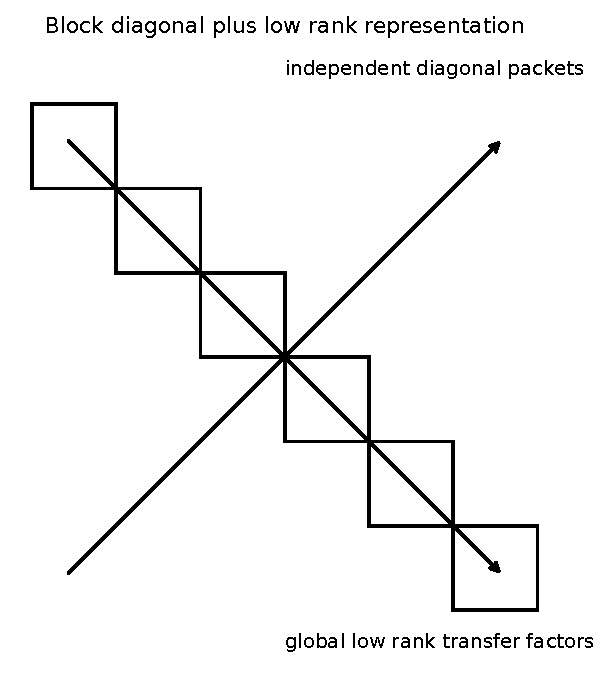
\includegraphics[width=.68\textwidth]{05_bdlr_structure.pdf}
\caption{A regular diagonal packet structure is coupled by global low rank factors.}
\label{fig:bdlr_structure}
\end{figure}

\subsection{Products and inverses}

\begin{theorem}[Exact BDLR product]\label{thm:bdlr_product}
Let
\[
A=D_A+U_AV_A^*,
\qquad
B=D_B+U_BV_B^*
\]
use the same diagonal packet layout. Then
\[
AB=D_AD_B+U_CV_C^*,
\]
where
\[
U_C
=
\begin{bmatrix}
D_AU_B+U_A(V_A^*U_B)&U_A
\end{bmatrix}
\]
and
\[
V_C
=
\begin{bmatrix}
V_B&D_B^*V_A
\end{bmatrix}.
\]
The unrecompressed correction rank is at most \(r_A+r_B\).
\end{theorem}

\begin{proof}
Expand the product:
\[
AB
=
D_AD_B
+D_AU_BV_B^*
+U_AV_A^*D_B
+U_A(V_A^*U_B)V_B^*.
\]
The second and fourth terms share the right factor \(V_B^*\). The third term equals
\[
U_A(D_B^*V_A)^*.
\]
Concatenation gives the stated factors.
\end{proof}

\begin{corollary}[Rank growth in a product chain]\label{cor:rank_growth}
Let
\[
A_j=D_j+U_jV_j^*,
\qquad
j=1,\ldots,m,
\]
share one diagonal packet layout. Before recompression, the product
\[
A_m\cdots A_1
\]
has a BDLR representation whose correction rank is at most
\[
\boxed{
\sum_{j=1}^m r_j.
}
\]
\end{corollary}

\begin{proof}
Apply \cref{thm:bdlr_product} inductively. Each new factor adds at most its own correction rank.
\end{proof}

\begin{theorem}[Woodbury inversion]\label{thm:woodbury}
Assume \(D\) and
\[
S=I+V^*D^{-1}U
\]
are invertible. Then
\[
\boxed{
(D+UV^*)^{-1}
=
D^{-1}
-D^{-1}US^{-1}V^*D^{-1}.
}
\]
\end{theorem}

\begin{proof}
Multiply the proposed inverse by \(D+UV^*\). The coefficient of \(V^*D^{-1}\) is
\[
U-US^{-1}(I+V^*D^{-1}U)=0.
\]
The remaining term is the identity. The right inverse calculation is the same.
\end{proof}

The formula and its history are discussed in \cite{Hager1989}. It reduces one large solve to packet solves with \(D\) and one dense solve with the small matrix \(S\).

\begin{corollary}[Inverse norm bound]\label{cor:inverse_norm}
Under the hypotheses of \cref{thm:woodbury},
\[
\norm{(D+UV^*)^{-1}}
\leq
\norm{D^{-1}}
+
\norm{D^{-1}U}
\norm{S^{-1}}
\norm{V^*D^{-1}}.
\]
\end{corollary}

\begin{proof}
Apply the triangle inequality and submultiplicativity to the Woodbury formula.
\end{proof}

\subsection{Optimal factor recompression}

\begin{standardfact}[Eckart Young Mirsky theorem]\label{fact:eym}
If \(M\) has singular values
\[
\sigma_1\geq\sigma_2\geq\cdots,
\]
then its truncated singular value decomposition \(M_k\) is a best rank at most \(k\) approximation. It satisfies
\[
\norm{M-M_k}_2=\sigma_{k+1}
\]
and
\[
\norm{M-M_k}_{\rm F}
=
\left(
\sum_{j>k}\sigma_j^2
\right)^{1/2}.
\]
\end{standardfact}

This is classical \cite{EckartYoung1936,Mirsky1960}. The next theorem shows that an \(n\) dimensional singular value decomposition is unnecessary when a correction is already factored.

\begin{theorem}[Small core recompression]\label{thm:small_core_recompression}
Let
\[
L\in\CC^{m\times r},
\qquad
R\in\CC^{n\times r}.
\]
Take compact QR factorizations
\[
L=Q_LR_L,
\qquad
R=Q_RR_R,
\]
where the columns of \(Q_L\) and \(Q_R\) are orthonormal. Form the small core
\[
G=R_LR_R^*
\]
and let
\[
G=W\Sigma Z^*
\]
be a singular value decomposition. Define
\[
L_k=Q_LW_k\Sigma_k^{1/2},
\qquad
R_k=Q_RZ_k\Sigma_k^{1/2}.
\]
Then
\[
L_kR_k^*
\]
is a best rank at most \(k\) approximation to \(LR^*\). Its spectral and Frobenius errors are the singular value tails in \cref{fact:eym}. The core dimensions equal the column ranks of the two input factors. A noncompact reduced QR may retain extra zero singular directions without changing the conclusion.
\end{theorem}

\begin{proof}
The exact factor product is
\[
LR^*
=
Q_LGQ_R^*.
\]
The two outer maps are isometries on their column spaces. They preserve the nonzero singular values and every unitarily invariant norm of the core. Truncating the singular value decomposition of \(G\) and applying \cref{fact:eym} gives the result. The compact QR dimensions equal the ranks of the factor column spaces.
\end{proof}

\begin{figure}[t]
\centering
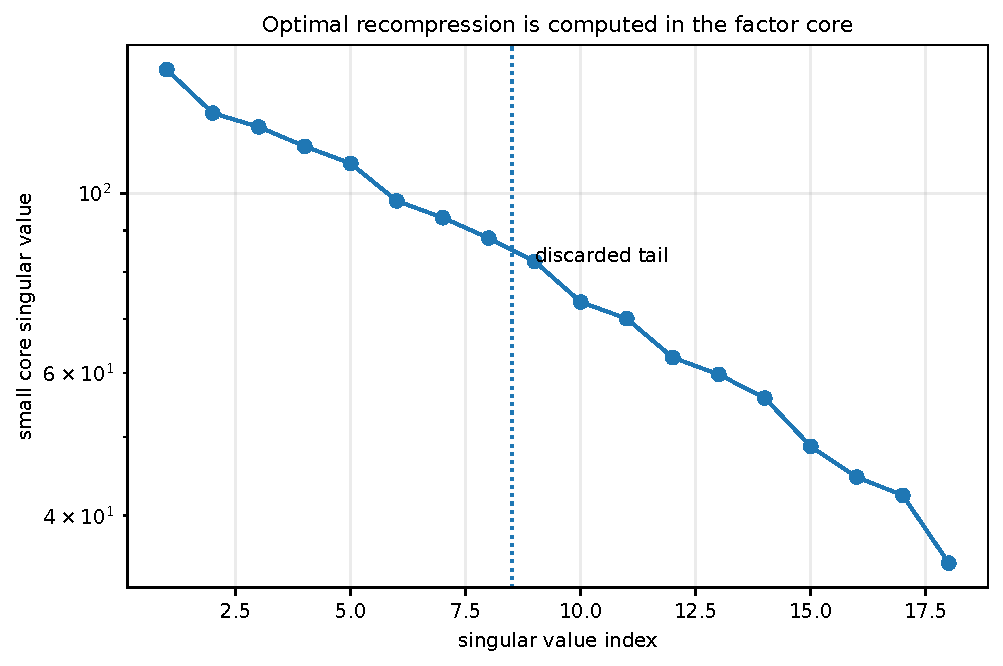
\includegraphics[width=.76\textwidth]{06_recompression_spectrum.pdf}
\caption{The approximation decision is made from the singular values of a small core whose dimension is the unrecompressed rank.}
\label{fig:recompression}
\end{figure}

\begin{remark}\label{rem:recompression_work}
The large matrices enter through QR factorizations of the factors. The singular value problem has dimension at most the unrecompressed rank. Updating and recompressing low rank factors is standard numerical linear algebra \cite{GolubKahan1965,BunchNielsen1978}.
\end{remark}

\begin{theorem}[Product chain perturbation]\label{thm:product_chain_error}
Let \(A_1,\ldots,A_m\) be exact factors and let
\[
\widehat A_j=A_j+E_j.
\]
Then
\[
\boxed{
\left\|
\widehat A_m\cdots\widehat A_1
-
A_m\cdots A_1
\right\|
\leq
\sum_{j=1}^m
\left(
\prod_{i=j+1}^m\norm{\widehat A_i}
\right)
\norm{E_j}
\left(
\prod_{i=1}^{j-1}\norm{A_i}
\right).
}
\]
Empty products are one.
\end{theorem}

\begin{proof}
Use the telescoping identity
\[
\widehat A_m\cdots\widehat A_1
-A_m\cdots A_1
=
\sum_{j=1}^m
\widehat A_m\cdots\widehat A_{j+1}
E_j
A_{j-1}\cdots A_1.
\]
Take norms term by term.
\end{proof}

\begin{theorem}[Certified repeated recompression]\label{cor:recompression_chain}
Let
\[
P_0=I,
\qquad
P_j=A_jP_{j-1},
\]
be exact partial products. Suppose an implemented chain satisfies
\[
\widehat P_0=I,
\qquad
\widehat P_j
=
A_j\widehat P_{j-1}+E_j,
\]
where \(E_j\) is the additive error introduced after the \(j\)th multiplication, for example by factor recompression. Then
\[
\boxed{
\norm{\widehat P_m-P_m}
\leq
\sum_{j=1}^{m}
\left(
\prod_{i=j+1}^{m}\norm{A_i}
\right)
\norm{E_j}.
}
\]
If \(\norm{E_j}\leq\delta_j\), the same formula with \(\delta_j\) gives a certified final error.
\end{theorem}

\begin{proof}
Set \(D_j=\widehat P_j-P_j\). Then
\[
D_j=A_jD_{j-1}+E_j,
\qquad
D_0=0.
\]
Repeated substitution gives
\[
D_m
=
\sum_{j=1}^{m}
A_mA_{m-1}\cdots A_{j+1}E_j.
\]
Taking norms yields the result.
\end{proof}

\section{Sparse transfer graphs and schedules}\label{sec:graphs}

\subsection{Support under algebraic operations}

\begin{theorem}[Path support of powers]\label{thm:path_support}
For every positive integer \(m\),
\[
P_\gamma A^mP_\alpha
\]
is the sum over directed paths
\[
\alpha=\alpha_0
\longrightarrow
\alpha_1
\longrightarrow\cdots\longrightarrow
\alpha_m=\gamma
\]
in \(G_A\), with contribution
\[
A_{\alpha_m\alpha_{m-1}}
\cdots
A_{\alpha_1\alpha_0}.
\]
If no such path exists, the block vanishes.
\end{theorem}

\begin{proof}
Insert the packet identity between every two consecutive factors of \(A\). Every nonzero term determines one path of length \(m\).
\end{proof}

\begin{corollary}[Polynomial support]\label{cor:polynomial_support}
If
\[
p(z)=\sum_{j=0}^dc_jz^j,
\]
then
\[
\supp(p(A))
\]
is contained in the union of the support relations of \(A^j\) for \(0\leq j\leq d\).
\end{corollary}

\begin{proof}
Apply \cref{thm:path_support} to every power in the polynomial.
\end{proof}

\begin{corollary}[Acyclic transfer nilpotence]\label{cor:acyclic_nilpotence}
Let \(K\) contain only strict transfer blocks. If its support graph is acyclic and its longest directed path has \(h\) edges, then
\[
K^{h+1}=0.
\]
\end{corollary}

\begin{proof}
There is no directed path of length \(h+1\). Every block of \(K^{h+1}\) therefore vanishes by \cref{thm:path_support}.
\end{proof}

\begin{figure}[t]
\centering
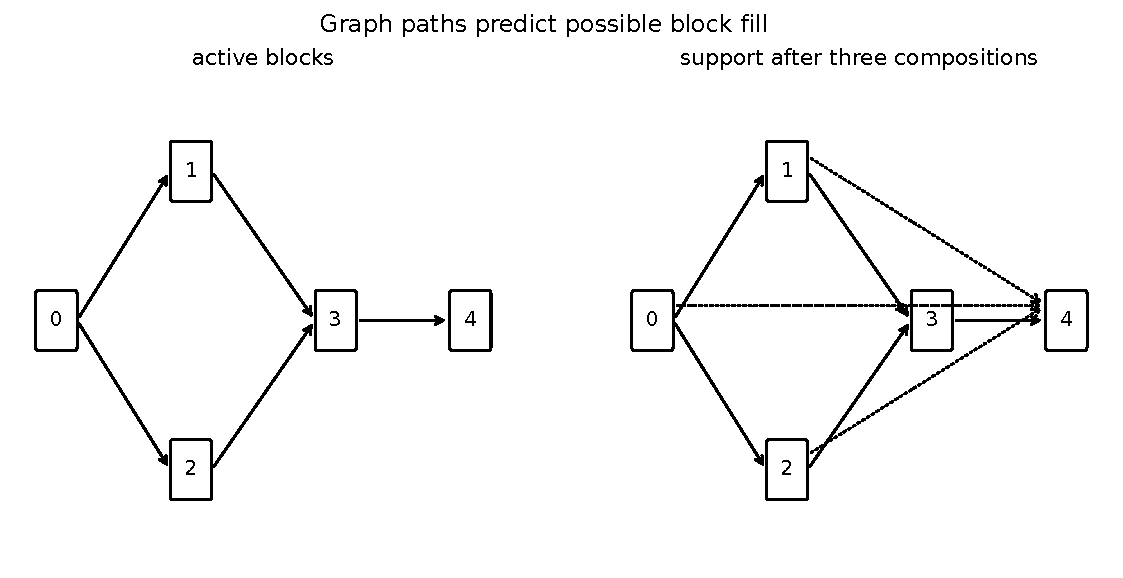
\includegraphics[width=.9\textwidth]{07_path_support.pdf}
\caption{Composition creates possible support along directed paths. Cancellation can remove an allowed block, so the graph gives an inclusion rather than an equality.}
\label{fig:path_support}
\end{figure}

\subsection{Block triangular solves}

\begin{definition}[Topological level]\label{def:topological_level}
Let \(G\) be a directed acyclic graph. The first level contains its source vertices. Remove them. The next level contains the new sources. Continue until every vertex has been assigned.
\end{definition}

\begin{theorem}[Level schedule for a triangular solve]\label{thm:level_schedule}
Let \(A=D+K\) be block lower triangular after a topological ordering. Assume every diagonal block \(D_\alpha\) is invertible. The solve
\[
Ax=b
\]
can be completed in one sequential stage per topological level. Blocks in the same level may be solved independently after all earlier levels are known.
\end{theorem}

\begin{proof}
The equation in packet \(\beta\) is
\[
D_\beta x_\beta
=
b_\beta
-
\sum_{\alpha\to\beta}K_{\beta\alpha}x_\alpha.
\]
Every predecessor of \(\beta\) lies in an earlier level. Once those values are available, \(x_\beta\) is obtained from the local solve with \(D_\beta\). Vertices in the same level have no directed edge between them, so their solves are independent.
\end{proof}

\begin{corollary}[Sequential depth]\label{cor:sequential_depth}
The number of sequential stages in the level schedule equals one plus the length of the longest directed path.
\end{corollary}

\begin{proof}
The recursive level of a vertex is one plus the largest level of its predecessors. The largest level therefore counts the vertices on a longest path.
\end{proof}

\begin{figure}[t]
\centering
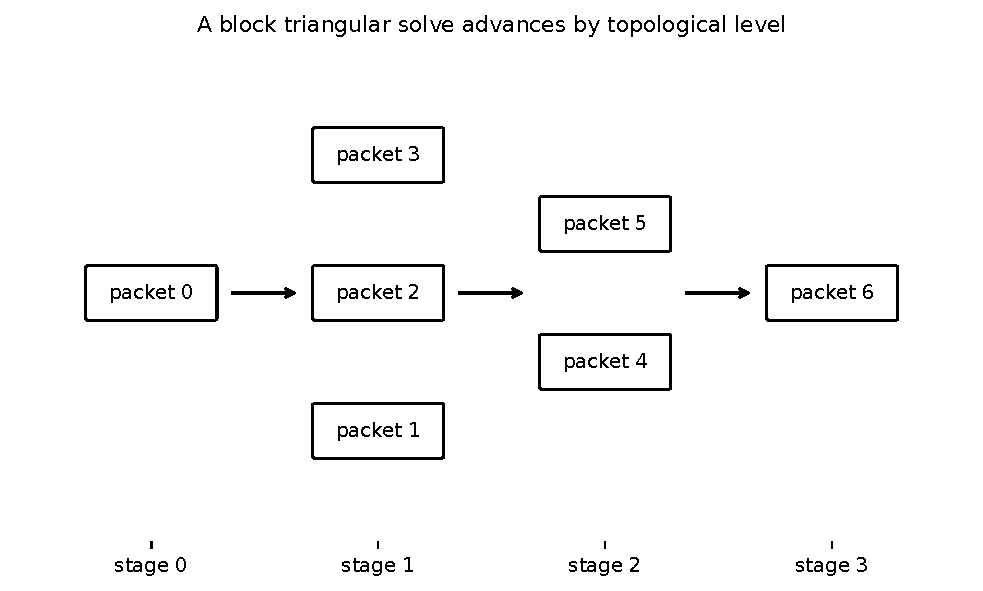
\includegraphics[width=.82\textwidth]{08_topological_schedule.pdf}
\caption{Packets in the same topological level can be processed concurrently in a triangular solve.}
\label{fig:topological_schedule}
\end{figure}

\subsection{Fill under elimination}

\begin{theorem}[Inverse support lies in the transitive closure]\label{thm:inverse_support}
Let \(A\) be an invertible packet operator. If there is no directed path from packet \(\alpha\) to packet \(\beta\) in \(G_A\), then
\[
\boxed{
P_\beta A^{-1}P_\alpha=0.
}
\]
\end{theorem}

\begin{proof}
Let \(R\) be the set of packets reachable from \(\alpha\), including \(\alpha\), and set
\[
X_R=\bigoplus_{\gamma\in R}X_\gamma.
\]
No active edge leaves \(R\), so \(AX_R\subseteq X_R\). The restriction of \(A\) to the finite dimensional space \(X_R\) is injective. It is therefore onto \(X_R\). Hence \(A^{-1}X_R\subseteq X_R\). Since \(\beta\notin R\), the stated block of \(A^{-1}\) vanishes.
\end{proof}

\begin{proposition}[Schur support inclusion]\label{prop:schur_fill}
Split the packets into retained indices \(R\) and hidden indices \(H\). Suppose the hidden block \(A_{HH}\) is invertible. The retained Schur complement is
\[
S
=
A_{RR}
-
A_{RH}A_{HH}^{-1}A_{HR}.
\]
A retained block \((\beta,\alpha)\) can be active only if it was already active in \(A_{RR}\), or if there is a directed walk from \(\alpha\) through hidden packets to \(\beta\).
\end{proposition}

\begin{proof}
The correction block is
\[
P_\beta A_{RH}A_{HH}^{-1}A_{HR}P_\alpha.
\]
It can be nonzero only when \(A_{HR}P_\alpha\) enters a hidden packet, the inverse hidden operator connects hidden packets, and \(P_\beta A_{RH}\) exits to \(\beta\). By \cref{thm:inverse_support}, the hidden inverse can connect only packets joined by a hidden directed path. Cancellation may still remove an allowed block.
\end{proof}

Sparse elimination and fill are treated systematically in \cite{Davis2006}. The packet graph records the same structural issue at block scale.

\section{Krylov methods and packet preconditioning}\label{sec:krylov}

\begin{definition}[Krylov space]\label{def:krylov}
For a linear operator \(A\), a vector \(v\), and a positive integer \(m\), define
\[
\Kcal_m(A,v)
=
\operatorname{span}
\{v,Av,\ldots,A^{m-1}v\}.
\]
\end{definition}

\begin{proposition}[Invariant packet Krylov decomposition]\label{prop:krylov_invariant}
Assume
\[
[A,P_\alpha]=0
\]
for every packet. If
\[
v=\sum_\alpha v_\alpha,
\qquad
v_\alpha=P_\alpha v,
\]
then
\[
A^jv
=
\sum_\alpha A_\alpha^jv_\alpha
\]
for every \(j\geq0\), where
\[
A_\alpha=P_\alpha AP_\alpha.
\]
Hence
\[
\Kcal_m(A,v)
\subseteq
\bigoplus_\alpha
\Kcal_m(A_\alpha,v_\alpha).
\]
\end{proposition}

\begin{proof}
Commutation gives
\[
A^jP_\alpha=P_\alpha A^j.
\]
Apply this identity to each packet component of \(v\).
\end{proof}

\begin{theorem}[Approximate packet Krylov bound]\label{thm:approx_krylov}
Write
\[
A=D+K,
\]
where \(D\) is packet diagonal. For every positive integer \(j\),
\[
\boxed{
\norm{A^j-D^j}
\leq
jM^{j-1}\norm{K},
}
\]
where
\[
M=\max\{\norm{A},\norm{D}\}.
\]
Consequently,
\[
\dist(A^jv,\bigoplus_\alpha\Kcal_{j+1}(D_\alpha,v_\alpha))
\leq
jM^{j-1}\norm{K}\norm{v}.
\]
\end{theorem}

\begin{proof}
Use the telescoping identity
\[
A^j-D^j
=
\sum_{k=0}^{j-1}
A^{j-1-k}KD^k.
\]
Each term has norm at most \(M^{j-1}\norm{K}\). The vector \(D^jv\) lies in the direct sum of local Krylov spaces.
\end{proof}

\begin{theorem}[Block Jacobi condition bound]\label{thm:block_jacobi}
Let
\[
A=D+K
\]
be Hermitian positive definite with positive block diagonal part \(D\). Suppose
\[
E=D^{-1/2}KD^{-1/2}
\]
is Hermitian and
\[
\norm{E}_2\leq\eta<1.
\]
Then
\[
\boxed{
\cond_2(D^{-1/2}AD^{-1/2})
\leq
\frac{1+\eta}{1-\eta}.
}
\]
\end{theorem}

\begin{proof}
For every unit vector \(x\),
\[
\abs{x^*Ex}\leq\eta.
\]
The Rayleigh quotient of \(I+E\) lies in \([1-\eta,1+\eta]\). The quotient of the extreme eigenvalue bounds gives the result.
\end{proof}

\begin{standardfact}[Preconditioned conjugate gradient convergence]\label{fact:cg}
Let \(A\) and \(M\) be Hermitian positive definite, and set
\[
\kappa
=
\cond_2(M^{-1/2}AM^{-1/2}).
\]
The energy norm error of preconditioned conjugate gradient satisfies
\[
\norm{x_m-x_*}_A
\leq
2
\left(
\frac{\sqrt\kappa-1}{\sqrt\kappa+1}
\right)^m
\norm{x_0-x_*}_A.
\]
\end{standardfact}

This standard estimate is discussed in \cite{Saad2003}. Combining it with \cref{thm:block_jacobi} yields an explicit iteration certificate when the normalized cross packet coupling is small.

\begin{figure}[t]
\centering
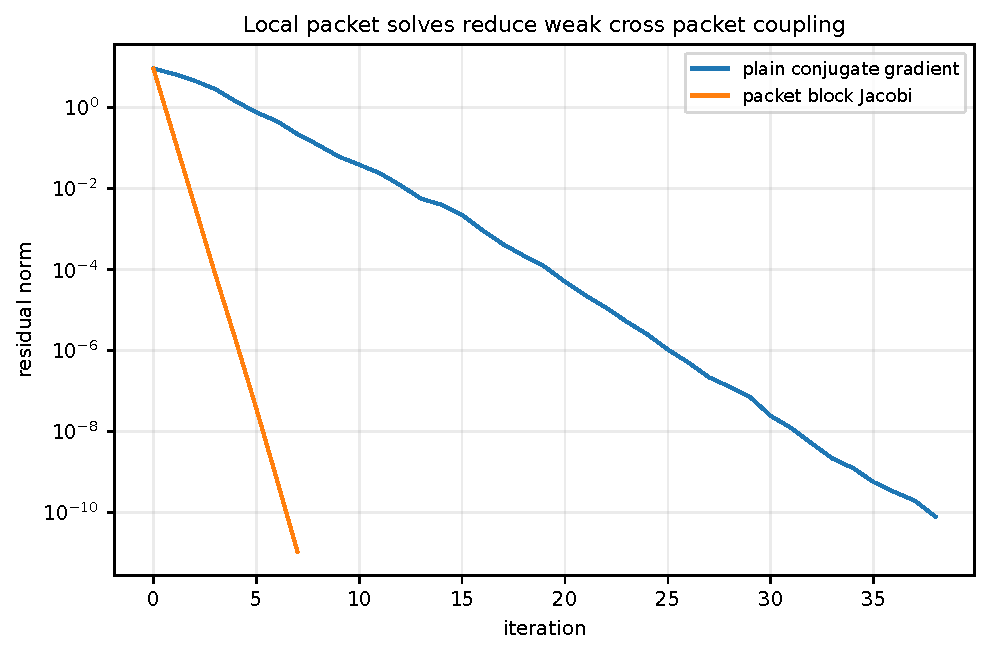
\includegraphics[width=.75\textwidth]{09_packet_preconditioner.pdf}
\caption{The block diagonal packet operator serves as a reusable local preconditioner in a weakly coupled positive system.}
\label{fig:preconditioner}
\end{figure}

\begin{corollary}[Certified packet preconditioning]\label{cor:certified_pcg}
Under the hypotheses of \cref{thm:block_jacobi}, the convergence factor in \cref{fact:cg} is bounded by the value obtained from
\[
\kappa
=
\frac{1+\eta}{1-\eta}.
\]
\end{corollary}

\begin{proof}
Insert the condition bound from \cref{thm:block_jacobi} into the monotone convergence factor in \cref{fact:cg}.
\end{proof}

\section{Packetwise mixed precision}\label{sec:precision}

\subsection{One operator}

\begin{theorem}[Packet perturbation certificate]\label{thm:packet_error}
Let
\[
A=
\sum_{e\in E}A_e,
\qquad
\widehat A
=
\sum_{e\in E}(A_e+E_e),
\]
where edge \(e\) starts at packet \(\alpha(e)\), and assume
\[
A_e=A_eP_{\alpha(e)},
\qquad
E_e=E_eP_{\alpha(e)}.
\]
Then
\[
\boxed{
\norm{(\widehat A-A)x}
\leq
\sum_{e\in E}
\norm{E_e}
\norm{P_{\alpha(e)}x}.
}
\]
If
\[
\norm{E_e}
\leq
\eps_e\norm{A_e},
\]
then
\[
\boxed{
\norm{(\widehat A-A)x}
\leq
\sum_{e\in E}
\eps_e\norm{A_e}
\norm{P_{\alpha(e)}x}.
}
\]
\end{theorem}

\begin{proof}
Exact packet evaluation gives
\[
(\widehat A-A)x
=
\sum_eE_eP_{\alpha(e)}x.
\]
Apply the triangle inequality and the operator norm bound to each term.
\end{proof}

\begin{standardfact}[Floating point matrix product model]\label{fact:rounding}
Under the standard floating point model, a computed matrix product may be written as an exact product with a dimension dependent backward perturbation. The perturbation constant is controlled by the unit roundoff and the inner dimension when overflow and underflow are excluded.
\end{standardfact}

Detailed forms and their hypotheses are given in \cite{Higham2002}. Packetwise use of this fact produces edge bounds \(\eps_e\) for \cref{thm:packet_error}.

\subsection{Several operators}

\begin{corollary}[Mixed precision product chain]\label{cor:mixed_chain}
If each factor \(A_j\) is replaced by a packetwise approximation \(\widehat A_j\), then the final operator error is bounded by \cref{thm:product_chain_error}. Each \(\norm{E_j}\) may in turn be bounded by the packet certificate in \cref{thm:packet_error}.
\end{corollary}

\begin{proof}
Apply \cref{thm:packet_error} at every stage and substitute the resulting operator error bounds into \cref{thm:product_chain_error}.
\end{proof}

\subsection{Continuous allocation}

\begin{theorem}[Continuous precision allocation]\label{thm:continuous_precision}
Let \(s_e>0\) be sensitivities and \(c_e>0\) be costs. Consider
\[
\min_{\eps_e>0}
\sum_e c_e\log\frac1{\eps_e}
\]
subject to
\[
\sum_es_e\eps_e=\tau.
\]
The unique minimizer is
\[
\boxed{
\eps_e
=
\frac{\tau c_e}{s_e\sum_fc_f}.
}
\]
\end{theorem}

\begin{proof}
The Lagrangian derivative gives
\[
-\frac{c_e}{\eps_e}+\lambda s_e=0.
\]
Thus
\[
\eps_e=\frac{c_e}{\lambda s_e}.
\]
The constraint gives
\[
\lambda=\frac{\sum_fc_f}{\tau}.
\]
The objective is strictly convex on the positive orthant, so the stationary point is the unique minimizer.
\end{proof}

\begin{theorem}[Clipped precision allocation]\label{thm:clipped_precision}
Add upper bounds
\[
0<\eps_e\leq m_e.
\]
Assume
\[
0<\tau\leq\sum_es_em_e.
\]
There is a unique \(\lambda>0\), except at the maximal tolerance endpoint, such that
\[
\boxed{
\eps_e
=
\min\left\{
m_e,
\frac{c_e}{\lambda s_e}
\right\}
}
\]
and
\[
\sum_es_e\eps_e=\tau.
\]
This vector minimizes the same objective over the clipped feasible set.
\end{theorem}

\begin{proof}
The Karush Kuhn Tucker conditions give the unconstrained form on every nonactive coordinate and equality with \(m_e\) on every active upper bound. The weighted sum
\[
\phi(\lambda)
=
\sum_es_e
\min\left\{
m_e,
\frac{c_e}{\lambda s_e}
\right\}
\]
is continuous and nonincreasing. It decreases from the maximal feasible value to zero. The constraint determines \(\lambda\). Strict convexity gives uniqueness of the minimizer.
\end{proof}

\begin{figure}[t]
\centering
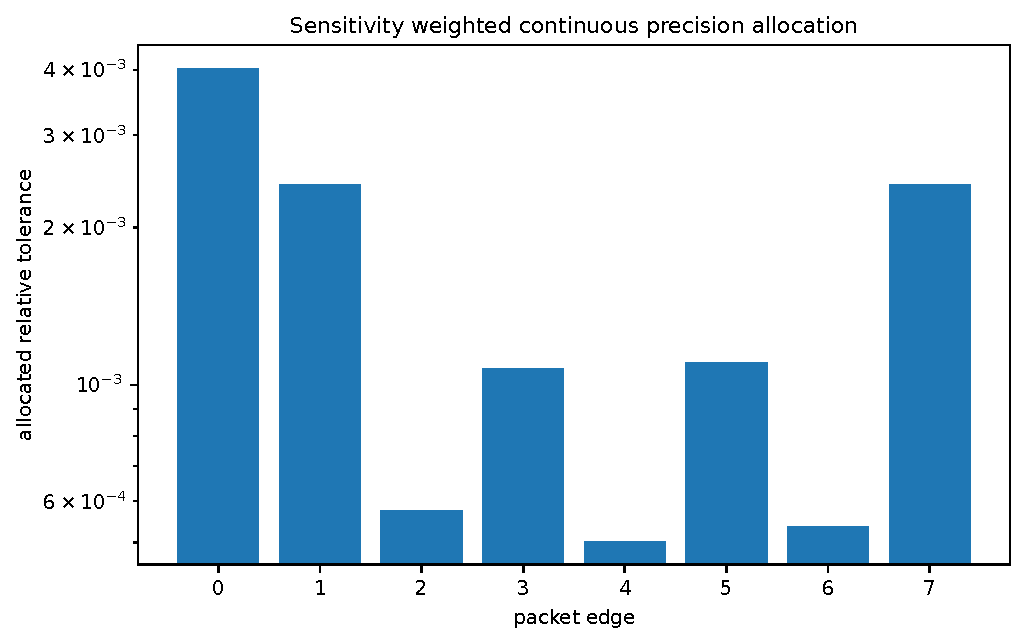
\includegraphics[width=.75\textwidth]{10_precision_allocation.pdf}
\caption{More sensitive packet edges receive tighter continuous tolerances.}
\label{fig:precision}
\end{figure}

\subsection{Discrete data types}

\begin{definition}[Discrete precision option]\label{def:dtype_option}
For edge \(e\), a discrete precision option \(k\) has a measured or modeled cost \(c_{e,k}\) and a nonnegative integer error weight \(w_{e,k}\). Exactly one option must be selected on every edge.
\end{definition}

\begin{theorem}[Exact discrete precision program]\label{thm:discrete_precision}
Let the total integer error budget be \(B\). Define
\[
F_j(b)
\]
as the minimum cost for assigning precisions to the first \(j\) edges with total weight exactly \(b\). Then
\[
F_0(0)=0,
\qquad
F_0(b)=+\infty
\quad\text{for }b\neq0.
\]
Set \(F_{j-1}(u)=+\infty\) whenever \(u<0\) or the state is unreachable. Then
\[
\boxed{
F_j(b)
=
\min_k
\left\{
F_{j-1}(b-w_{j,k})+c_{j,k}
\right\}.
}
\]
The minimum of \(F_m(b)\) over \(0\leq b\leq B\) is the exact minimum cost for the quantized model.
\end{theorem}

\begin{proof}
Every feasible assignment for the first \(j\) edges ends with one option \(k\) on edge \(j\). Removing it leaves an optimal or suboptimal assignment for the first \(j-1\) edges with residual weight \(b-w_{j,k}\). Replacing a suboptimal prefix by an optimal one can only lower cost. The recurrence therefore has optimal substructure. Induction on \(j\) proves the result.
\end{proof}

\begin{remark}\label{rem:dtype_boundary}
The discrete program is exact only for the supplied options and quantized error weights. Real kernels also depend on accumulation type, scaling, overflow, underflow, tensor core availability, and shape restrictions. Mixed precision iterative refinement has its own conditioning requirements \cite{CarsonHigham2018}.
\end{remark}

\section{Discovery and exact packet compilation}\label{sec:compiler}

\subsection{Exact spectral discovery}

\begin{standardfact}[Simultaneous spectral decomposition]\label{fact:simultaneous}
A finite family of pairwise commuting normal matrices admits a common orthonormal basis of joint eigenvectors. The joint eigenspaces associated with distinct eigenvalue tuples give the coarsest orthogonal packet system on which every matrix in the family acts as a scalar.
\end{standardfact}

\begin{proposition}[Exact block discovery certificate]\label{prop:block_discovery_certificate}
For an orthogonal packet system \((P_\alpha)\), define the block diagonal compression
\[
\Pi_{\Pcal}(A)
=
\sum_\alpha P_\alpha AP_\alpha.
\]
Then
\[
\boxed{
\norm{A-\Pi_{\Pcal}(A)}_{\rm F}^2
=
\sum_{\alpha\neq\beta}
\norm{P_\beta AP_\alpha}_{\rm F}^2.
}
\]
In operator norm,
\[
\boxed{
\norm{A-\Pi_{\Pcal}(A)}_2
\leq
\sum_{\alpha\neq\beta}
\norm{P_\beta AP_\alpha}_2.
}
\]
Thus any proposed packet discovery has an exact finite residual certificate after its projectors are known.
\end{proposition}

\begin{proof}
Distinct matrix blocks are orthogonal in the Hilbert Schmidt inner product. Their squared Frobenius norms therefore add. The operator norm estimate follows from the triangle inequality.
\end{proof}

This supplies one exact discovery regime and one exact a posteriori certificate. Perturbation of spectral packets requires a gap. The Davis Kahan theorem gives quantitative control for Hermitian spectral subspaces under such a gap \cite{DavisKahan1970}. Randomized low rank discovery supplies another controlled regime \cite{HalkoMartinssonTropp2011,MartinssonTropp2020}. Neither result gives globally optimal packet discovery for arbitrary operators.

\subsection{Candidate packet trees}

\begin{definition}[Candidate representation tree]\label{def:candidate_tree}
A candidate representation tree is a finite rooted tree. Every node \(v\) has
\[
\kappa_v\geq0,
\qquad
\epsilon_v\geq0,
\]
representing the cost and error of keeping \(v\) as one leaf. Every internal node also has a split overhead \(\sigma_v\geq0\). An admissible pruning contains exactly one selected node on every root to terminal path.
\end{definition}

The cost and error of a pruning \(\Lcal\) are
\[
\cost(\Lcal)
=
\sum_{v\in\Lcal}\kappa_v
+
\sum_{u\text{ split}}\sigma_u
\]
and
\[
\err(\Lcal)=\sum_{v\in\Lcal}\epsilon_v.
\]
The model can include arithmetic, storage, launch, transfer, and precision costs inside \(\kappa_v\). It remains exact only when the declared totals are additive.

\begin{theorem}[Exact Lagrangian packet compiler]\label{thm:tree_compiler}
Fix \(\lambda\geq0\) and define
\[
J_\lambda(\Lcal)
=
\cost(\Lcal)
+
\lambda\err(\Lcal).
\]
For every node \(v\), set
\[
K_\lambda(v)
=
\kappa_v+\lambda\epsilon_v
\]
and
\[
S_\lambda(v)
=
\sigma_v
+
\sum_{w\in\operatorname{child}(v)}F_\lambda(w).
\]
For a terminal node, set
\[
F_\lambda(v)=K_\lambda(v).
\]
For an internal node, the recurrence
\[
\boxed{
F_\lambda(v)
=
\min\{K_\lambda(v),S_\lambda(v)\}
}
\]
computes the exact minimum Lagrangian objective over every admissible pruning of the subtree rooted at \(v\).
\end{theorem}

\begin{proof}
A pruning of the subtree rooted at \(v\) has two possible forms. It keeps \(v\), in which case its objective is \(K_\lambda(v)\). Otherwise it splits \(v\) and independently chooses an admissible pruning in every child subtree. By induction, the optimal child values are \(F_\lambda(w)\). The split objective is therefore \(S_\lambda(v)\). Taking the smaller value is exact.
\end{proof}

This recurrence is a computational version of best basis selection and Bellman optimality \cite{Bellman1957,CoifmanWickerhauser1992}. The node costs here may include operator application, transfer, launch, precision, and output conversion rather than only a signal entropy.

\begin{figure}[t]
\centering
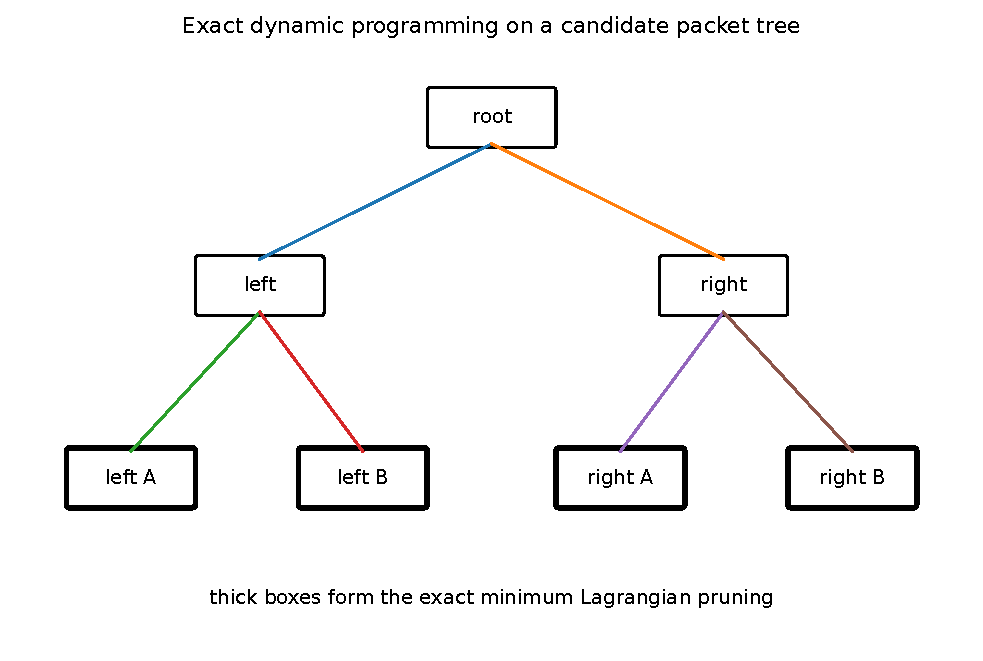
\includegraphics[width=.82\textwidth]{11_tree_compiler.pdf}
\caption{The thick leaves are selected by the exact Lagrangian recurrence.}
\label{fig:tree_compiler}
\end{figure}

\begin{corollary}[Shared compilation for an operator family]\label{cor:shared_compiler}
Let operators \(A^{(1)},\ldots,A^{(m)}\) use the same candidate tree. Give operator \(j\) a nonnegative reuse weight \(r_j\). Replace the local keep cost and error by
\[
\kappa_v
=
\kappa_v^{\rm setup}
+
\sum_{j=1}^m r_j\kappa_v^{(j)}
\]
and
\[
\epsilon_v
=
\sum_{j=1}^m r_j\epsilon_v^{(j)}.
\]
Then \cref{thm:tree_compiler} gives the exact optimal shared pruning for the additive weighted objective.
\end{corollary}

\begin{proof}
The weighted family objective is still the sum of local leaf and split terms. Apply \cref{thm:tree_compiler} to the aggregated quantities.
\end{proof}

\begin{proposition}[Monotone Lagrangian frontier]\label{prop:lagrangian_frontier}
Let \(0\leq\lambda_1<\lambda_2\). Choose optimal prunings \(\Lcal_1\) and \(\Lcal_2\) for the two Lagrangian parameters. Then
\[
\boxed{
\err(\Lcal_2)
\leq
\err(\Lcal_1)
}
\]
and
\[
\boxed{
\cost(\Lcal_2)
\geq
\cost(\Lcal_1).
}
\]
\end{proposition}

\begin{proof}
Optimality gives
\[
\cost(\Lcal_1)+\lambda_1\err(\Lcal_1)
\leq
\cost(\Lcal_2)+\lambda_1\err(\Lcal_2)
\]
and
\[
\cost(\Lcal_2)+\lambda_2\err(\Lcal_2)
\leq
\cost(\Lcal_1)+\lambda_2\err(\Lcal_1).
\]
Adding the inequalities yields
\[
(\lambda_2-\lambda_1)
\bigl(
\err(\Lcal_2)-\err(\Lcal_1)
\bigr)
\leq0.
\]
The error ordering follows. Substitution into the first inequality gives the cost ordering.
\end{proof}

\begin{corollary}[Supported Pareto points]\label{cor:supported_pareto}
For \(\lambda>0\), every Lagrangian optimum is Pareto optimal for the pair
\[
(\cost,\err).
\]
The quantized budget compiler may recover Pareto points that are not optimal for any Lagrangian parameter.
\end{corollary}

\begin{proof}
If another pruning had no larger cost and no larger error, with one strict inequality, its Lagrangian objective would be smaller. This contradicts optimality. A finite nonconvex frontier can contain points that are not supported by a line of slope \(-\lambda\), so the budget formulation is genuinely additional.
\end{proof}

\subsection{An exact error budget compiler}

\begin{theorem}[Quantized budget dynamic program]\label{thm:budget_compiler}
Assume every keep error is a nonnegative integer \(w_v\). Let \(B\in\NN\). For each node \(v\), define \(F_v(b)\) as the minimum cost of a pruning of the subtree at \(v\) with total error exactly \(b\). The keep option contributes
\[
F_v(w_v)\leq\kappa_v.
\]
The split option is obtained by min plus convolution of the child tables, followed by addition of \(\sigma_v\). The smallest value among
\[
F_{\rm root}(b),
\qquad
0\leq b\leq B,
\]
is the exact minimum cost among prunings whose quantized error is at most \(B\).
\end{theorem}

\begin{proof}
The keep case is immediate. In the split case, an admissible pruning is the union of one admissible pruning from each child. Its error is the sum of the child errors and its cost is the sum of their costs plus \(\sigma_v\). Repeated min plus convolution enumerates every possible distribution of the integer budget across the child subtrees. Induction on the tree proves exactness.
\end{proof}

\begin{corollary}[Pseudo polynomial complexity]\label{cor:budget_complexity}
If the maximum number of children is bounded and the budget is \(B\), the quantized compiler has pseudo polynomial complexity in the number of tree nodes and \(B\). A direct pairwise convolution implementation has quadratic dependence on \(B\) at each merge.
\end{corollary}

\begin{proof}
Every table has at most \(B+1\) entries. Merging two tables by direct convolution examines at most \((B+1)^2\) pairs. A bounded number of merges occurs at every node.
\end{proof}

\begin{figure}[t]
\centering
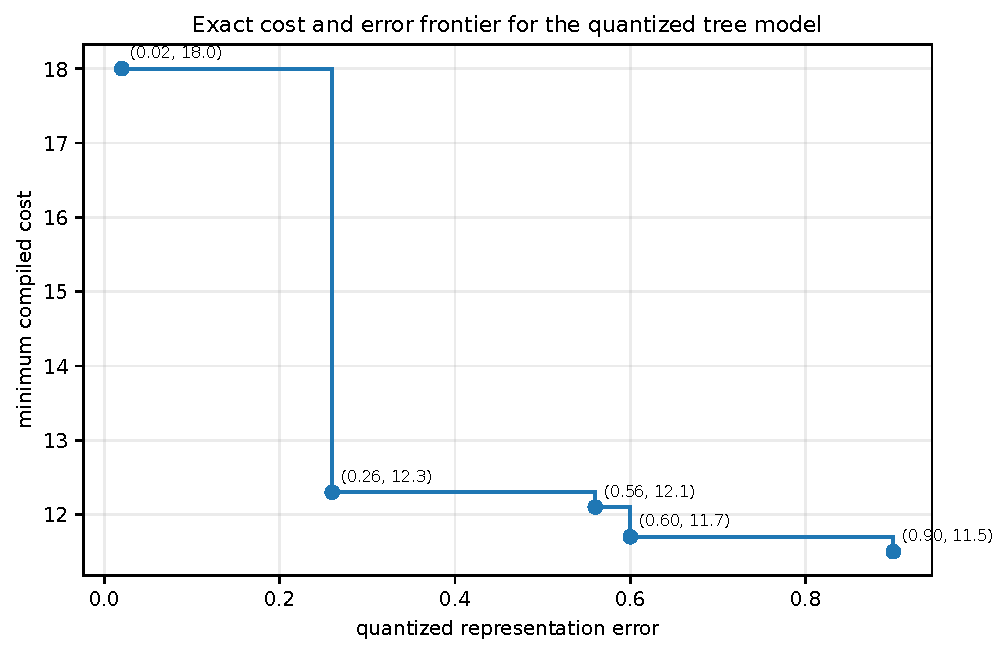
\includegraphics[width=.75\textwidth]{12_budget_compiler_frontier.pdf}
\caption{The quantized dynamic program produces the exact cost and error frontier for its finite model.}
\label{fig:budget_frontier}
\end{figure}

\subsection{Decision stability and local updates}

\begin{definition}[Decision gap]\label{def:decision_gap}
At an internal node \(v\), let
\[
g_v
=
\abs{K_\lambda(v)-S_\lambda(v)}.
\]
This is the gap between the keep and split scores after the child subproblems have been solved.
\end{definition}

\begin{theorem}[Compiler stability]\label{thm:compiler_stability}
Suppose the keep score and split score at every internal node change by less than \(g_v/2\). Then every strict keep or split decision in the original optimal pruning remains unchanged.
\end{theorem}

\begin{proof}
If the original keep score is lower by \(g_v\), then after perturbation it can increase by less than \(g_v/2\), while the split score can decrease by less than \(g_v/2\). The order remains strict. The split case is the same. Apply the argument from the leaves upward.
\end{proof}

\begin{theorem}[Local recompilation]\label{thm:local_recompilation}
Suppose local costs change only inside the subtree rooted at \(u\). Then every dynamic programming value outside that subtree and outside the ancestor chain from \(u\) to the root remains unchanged. Recomputing the subtree at \(u\) and that ancestor chain gives the exact new global optimum.
\end{theorem}

\begin{proof}
A node value depends only on its own local data and the values of its children. Nodes outside the changed subtree and outside the ancestor chain have the same local data and the same child values. Their values remain unchanged. Every affected dependency lies inside the changed subtree or on the unique path from \(u\) to the root.
\end{proof}

\begin{remark}[Boundary of the compiler theorem]\label{rem:compiler_boundary}
The exact compiler requires a finite candidate tree and additive local models. Arbitrary overlapping decompositions, nonlocal cache interactions, global rank coupling, and unrestricted structure discovery can destroy optimal substructure. No universal approximation factor is proved for those settings.
\end{remark}

\section{Device scheduling and amortization}\label{sec:scheduling}

\subsection{Shape classes}

\begin{definition}[Shape class]\label{def:shape_class}
Two active packet blocks lie in the same shape class when their input dimension, output dimension, right hand side count, scalar type, accumulation type, and kernel contract agree.
\end{definition}

\begin{proposition}[Launch reduction by shape]\label{prop:shape_launch}
Suppose \(B\) independent active blocks fall into \(g\) shape classes, and suppose the backend accepts one batched array or pointer list for each class. Grouped execution then requires at most \(g\) launches instead of \(B\), without changing the arithmetic or the output.
\end{proposition}

\begin{proof}
Place all blocks in one class along a batch dimension and invoke one batched kernel for that class. Every block receives the same local computation. One launch per class is sufficient.
\end{proof}

CUDA provides graph capture and replay for repeated dependency graphs \cite{NVIDIA2026}. These mechanisms reduce repeated launch work, but they do not change the operator or its arithmetic count.

\subsection{Critical path}

\begin{theorem}[Acyclic schedule depth]\label{thm:dag_depth}
Let a packet task graph be acyclic. Assume every task takes one normalized stage, every edge is a dependency, and an unlimited number of independent tasks may run concurrently. The minimum possible number of sequential stages equals the number of vertices on a longest directed path.
\end{theorem}

\begin{proof}
Every path gives a lower bound because its tasks must execute in order. The topological level schedule in \cref{thm:level_schedule} achieves exactly this depth.
\end{proof}

\subsection{One time costs}

\begin{theorem}[Amortization threshold]\label{thm:amortization}
Let \(s\geq0\) be a one time setup cost. Let \(t_b\) be the baseline time per use and \(t_c\) the candidate time per use. If \(t_b>t_c\), the candidate is faster after \(R\) uses exactly when
\[
R>
\frac{s}{t_b-t_c}.
\]
The smallest integer reuse count is
\[
\boxed{
R_{\min}
=
\left\lfloor
\frac{s}{t_b-t_c}
\right\rfloor+1.
}
\]
If \(t_b\leq t_c\), no positive reuse count amortizes a positive setup cost.
\end{theorem}

\begin{proof}
Compare
\[
s+Rt_c
\]
with
\[
Rt_b.
\]
Rearranging gives the stated inequality.
\end{proof}

\begin{corollary}[Graph replay threshold]\label{cor:graph_threshold}
If graph capture costs \(c\), ordinary execution costs \(t_o\), and replay costs \(t_r<t_o\), then capture is profitable when
\[
R>
\frac{c}{t_o-t_r}.
\]
\end{corollary}

\begin{proof}
Apply \cref{thm:amortization} with setup cost \(c\).
\end{proof}

\begin{corollary}[Materialization threshold]\label{cor:materialization_threshold}
Suppose a compressed representation costs \(t_c\) per downstream use, an explicit representation costs \(t_e\) per use, and one time materialization costs \(m\). Materialization is profitable only when
\[
R>
\frac{m}{t_c-t_e}
\]
and \(t_c>t_e\).
\end{corollary}

\begin{proof}
Compare repeated compressed use with materialization followed by repeated explicit use.
\end{proof}

\section{Benchmark contracts and measurement protocol}\label{sec:benchmark_protocol}

Performance data are meaningful only after the mathematical and timing contracts are fixed. The protocol follows standard concerns from numerical linear algebra, floating point analysis, and machine performance modeling \cite{Higham2002,GolubVanLoan2013,WilliamsWatermanPatterson2009}.

\begin{definition}[Case signature]\label{def:case_signature}
A case signature records the dimensions, packet layout, rank, right hand side count, random seed, source values, source type, reference computation, and output contract.
\end{definition}

\begin{definition}[Fair match]\label{def:fair_match}
Two measured rows are a fair match when they share one case signature, return the same declared output, use the same correctness reference, and have identical timing scopes. If one row includes an extra conversion or setup cost, it is a different scope and must be reported separately or added to both rows before comparison.
\end{definition}

\begin{proposition}[Fair matching is an equivalence relation]\label{prop:fair_equivalence}
On rows with complete metadata, equality of the case signature, output contract, correctness reference, and timing scope is an equivalence relation.
\end{proposition}

\begin{proof}
Equality of each metadata field is reflexive, symmetric, and transitive. Their conjunction has the same properties.
\end{proof}

\begin{definition}[Representation gain]\label{def:representation_gain}
Representation gain compares dense and structured work or storage for the same operator, independently of the processor.
\end{definition}

\begin{definition}[Device gain]\label{def:device_gain}
Device gain compares processors for the same representation, output, and timing scope.
\end{definition}

\begin{definition}[Kernel gain]\label{def:kernel_gain}
Kernel gain compares two implementations on the same device for the same representation, output, and timing scope.
\end{definition}

\begin{definition}[Amortization gain]\label{def:amortization_gain}
Amortization gain records the effect of one time discovery, compilation, transfer, capture, or materialization at a declared reuse count.
\end{definition}

A measured total speedup can mix these four effects. A multiplicative decomposition is only exact when matched rows isolate the factors. Otherwise the decomposition is interpretive.

\begin{figure}[t]
\centering
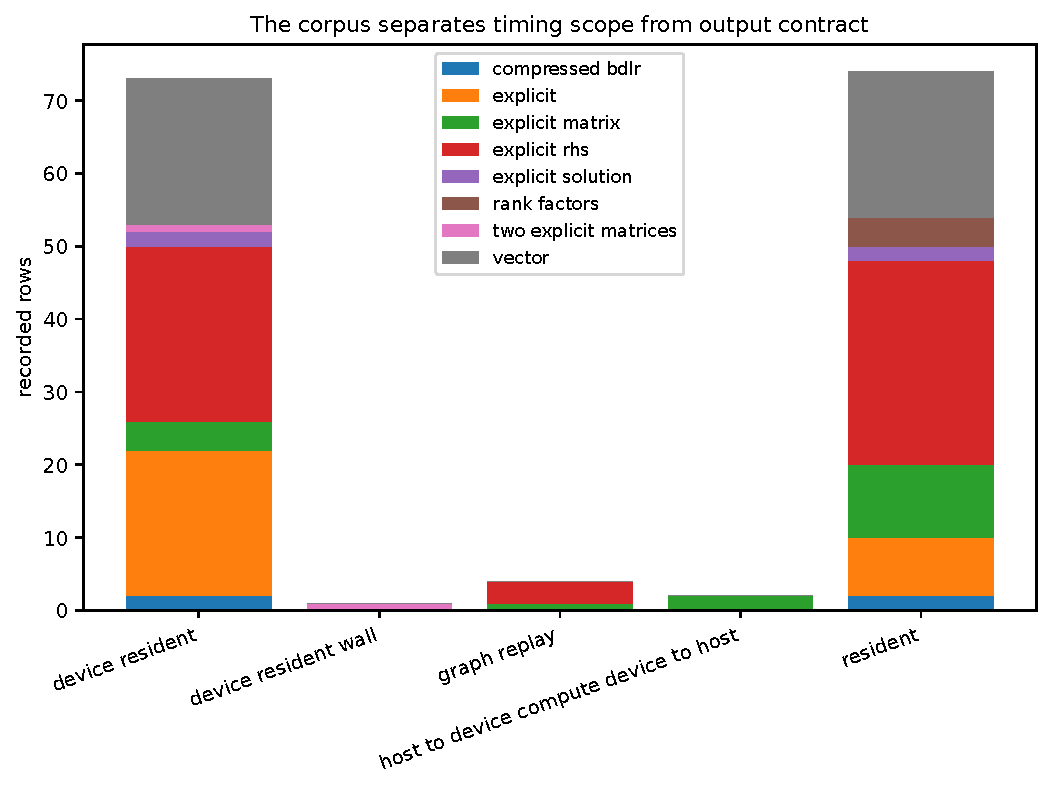
\includegraphics[width=.86\textwidth]{22_benchmark_contracts.pdf}
\caption{The corpus records timing scope and output contract as separate fields.}
\label{fig:contracts}
\end{figure}

\begin{remark}[Logical work rate]\label{rem:logical_gflops}
A structured method may report a dense equivalent logical work rate greater than the physical dense throughput because it does not execute the dense operations. This statistic describes avoided work. It is not a claim that the device performed those operations.
\end{remark}

\section{Recorded CPU and GPU corpus}\label{sec:measured}

The empirical corpus contains 154 measured rows from sixteen suites. It has 74 CPU rows and 80 GPU rows. The GPU was an NVIDIA GeForce RTX 3070 Ti Laptop GPU with compute capability 8.6 and 8 GB nominal memory. The recorded software used PyTorch 2.11.0 with a CUDA 12.8 build. These facts identify the environment. They do not predict another machine.

\begin{table}[t]
\centering
\small
\begin{tabular}{>{\raggedright\arraybackslash}p{.24\textwidth}r>{\raggedright\arraybackslash}p{.24\textwidth}r}
\toprule
Suite & Rows & Suite & Rows \\
\midrule
Dense multiplication & 28 & BDLR application & 15 \\
Block diagonal & 12 & BDLR product & 12 \\
Circulant & 12 & Toeplitz & 12 \\
Kronecker & 12 & Block banded & 8 \\
Sparse plus low rank & 8 & HODLR & 8 \\
Strassen & 6 & Transfer pipeline & 5 \\
Walsh Hadamard & 4 & Hidden blocks & 4 \\
Randomized low rank & 4 & Iterative refinement & 4 \\
\bottomrule
\end{tabular}
\caption{Coverage of the sanitized measured corpus.}
\label{tab:suites}
\end{table}

\subsection{Dense precision frontier}

At dimension \(4096\), the device resident dense rows gave the values in \cref{tab:dense_frontier}.

\begin{table}[t]
\centering
\small
\begin{tabular}{lrrr}
\toprule
Method & Median time in ms & Logical GFLOP per second & Relative error \\
\midrule
FP64 & 541.2803 & 253.91 & \(2.18\times10^{-15}\) \\
FP32 & 18.1309 & 7580.35 & \(5.76\times10^{-7}\) \\
TF32 & 8.6999 & 15797.75 & \(2.94\times10^{-4}\) \\
FP16 & 4.0264 & 34134.72 & \(3.60\times10^{-4}\) \\
BF16 & 4.1482 & 33132.00 & \(2.88\times10^{-3}\) \\
\bottomrule
\end{tabular}
\caption{Recorded dense accuracy and throughput at one dimension.}
\label{tab:dense_frontier}
\end{table}

\begin{figure}[t]
\centering
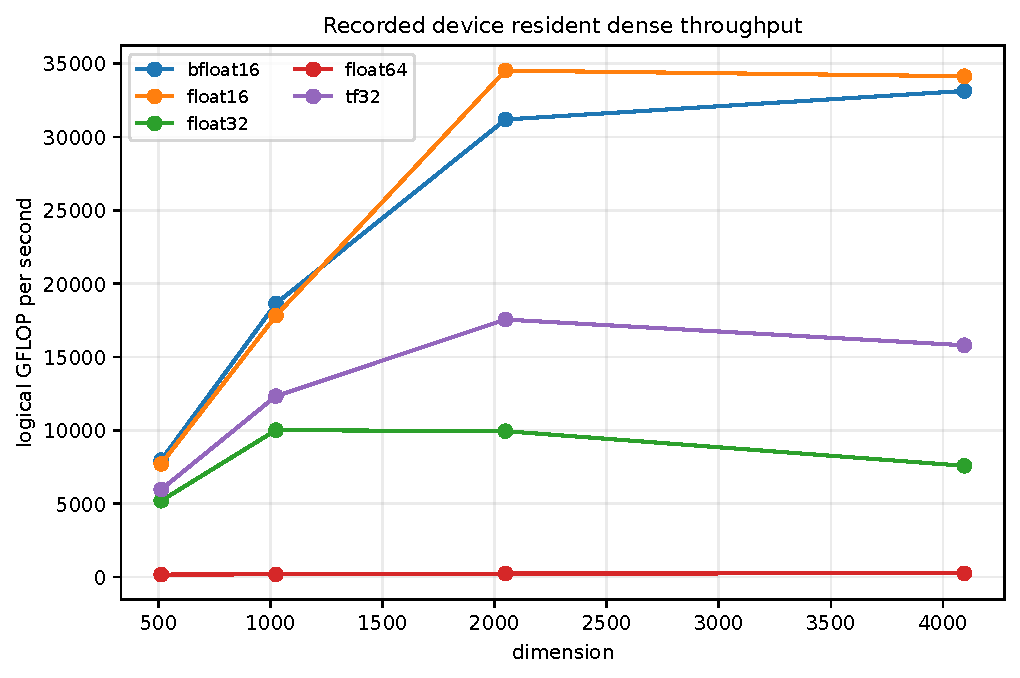
\includegraphics[width=.76\textwidth]{13_dense_gpu_throughput.pdf}
\caption{Recorded device resident dense throughput across dimensions and scalar types.}
\label{fig:dense_throughput}
\end{figure}

\begin{figure}[t]
\centering
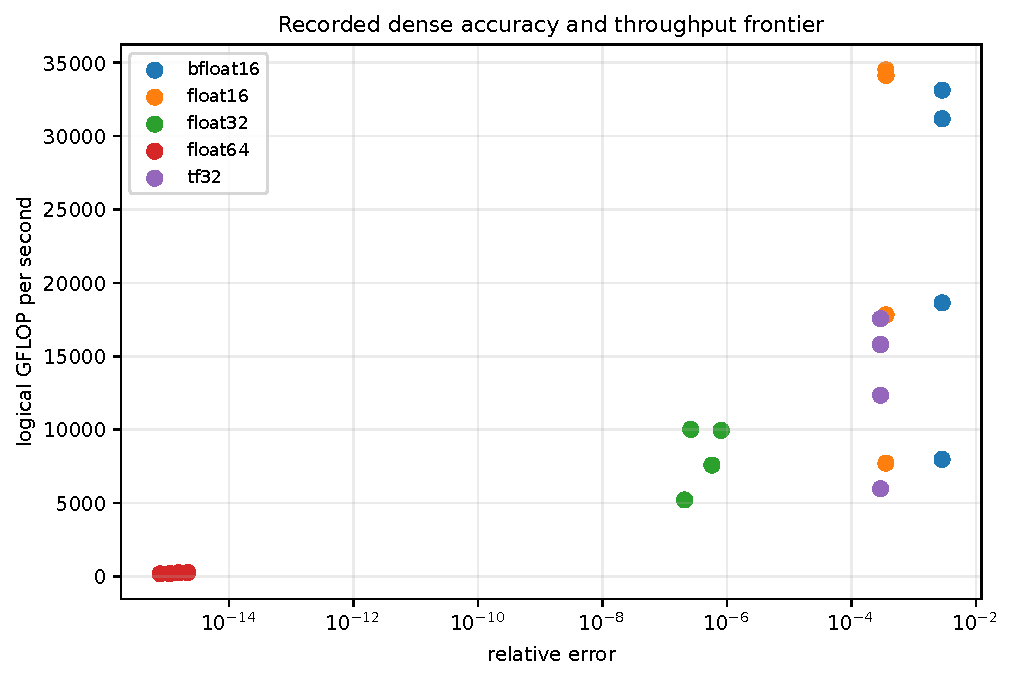
\includegraphics[width=.75\textwidth]{14_accuracy_frontier.pdf}
\caption{The speed and error tradeoff depends on both precision and problem size.}
\label{fig:accuracy_frontier}
\end{figure}

The frontier is not a universal ordering of scalar types. It records one generated family. Packet precision assignment should use local sensitivities and supported kernels rather than one global type.

\subsection{Regular packet operators}

For an \(8192\) by \(8192\) equal block operator with block width \(64\) and \(32\) right hand sides, the batched packet calculation took
\[
0.046032\text{ ms}.
\]
It was
\[
14.8919
\]
times faster than the matched device resident dense GPU row and
\[
235.7404
\]
times faster than the matched CPU dense row. The relative error was
\[
8.17\times10^{-8}.
\]

\begin{figure}[t]
\centering
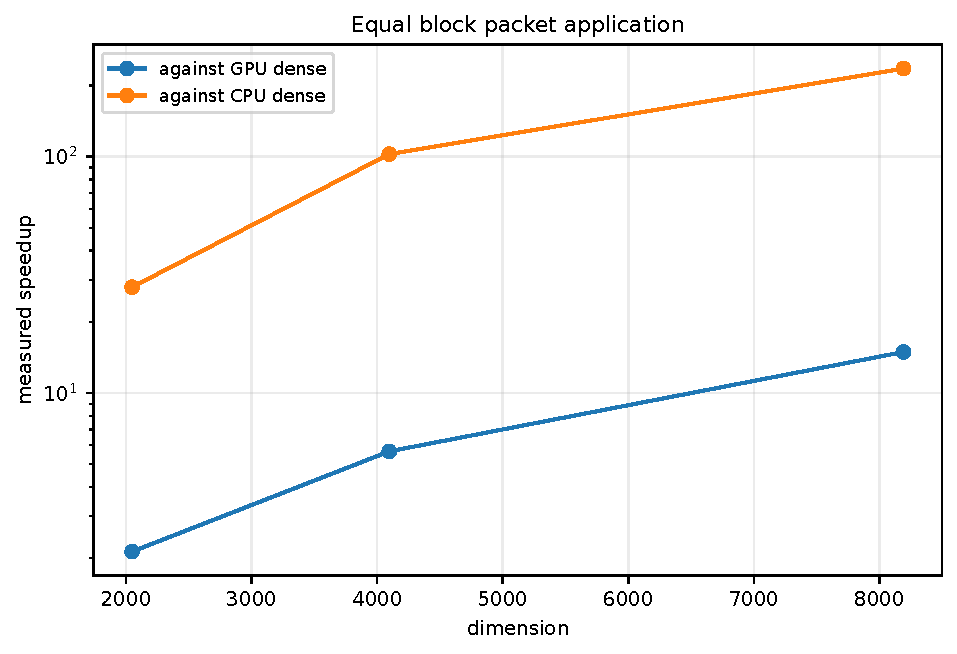
\includegraphics[width=.74\textwidth]{15_block_diagonal_speedup.pdf}
\caption{Regular equal shapes expose both representation reduction and batched execution.}
\label{fig:block_speedup}
\end{figure}

For BDLR application with the same dimension and right hand side count, block width \(64\), and rank \(8\), CUDA Graph replay took
\[
0.079872\text{ ms}.
\]
It was
\[
10.9355
\]
times faster than the matched dense GPU row and
\[
153.6527
\]
times faster than the matched CPU dense row. Capture time was excluded from the replay scope and must be amortized separately.

\begin{figure}[t]
\centering
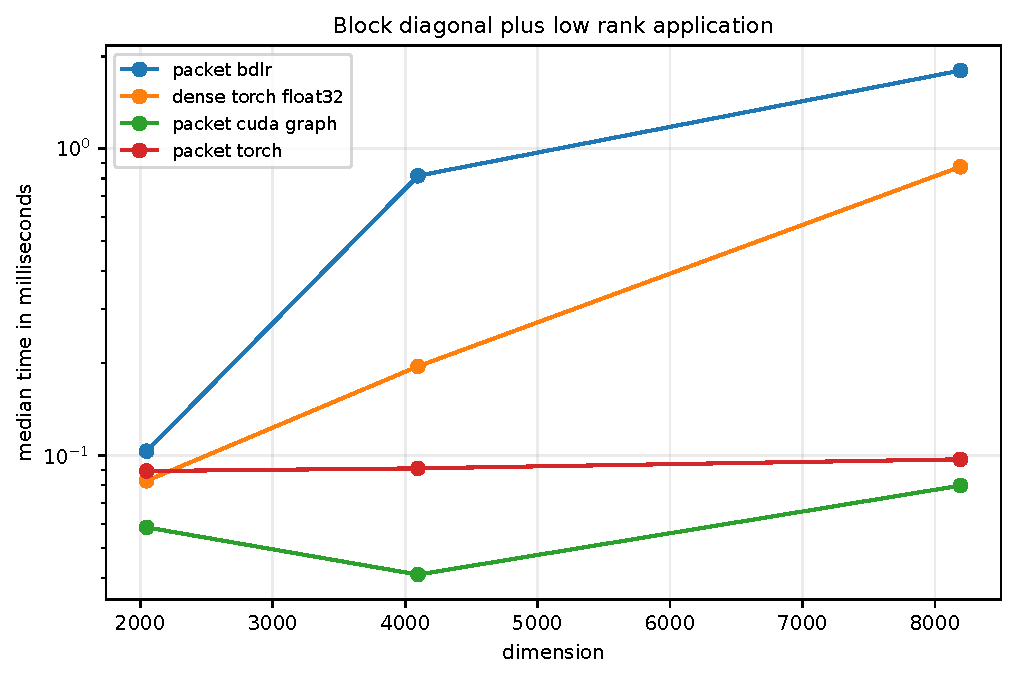
\includegraphics[width=.77\textwidth]{16_bdlr_timings.pdf}
\caption{Representation and launch strategy both affect BDLR application time.}
\label{fig:bdlr_timings}
\end{figure}

\subsection{Compressed products}

A compressed BDLR product returns block and low rank factors. Materialization returns all matrix entries. The measured product rows show the cost of changing the output contract.

\begin{figure}[t]
\centering
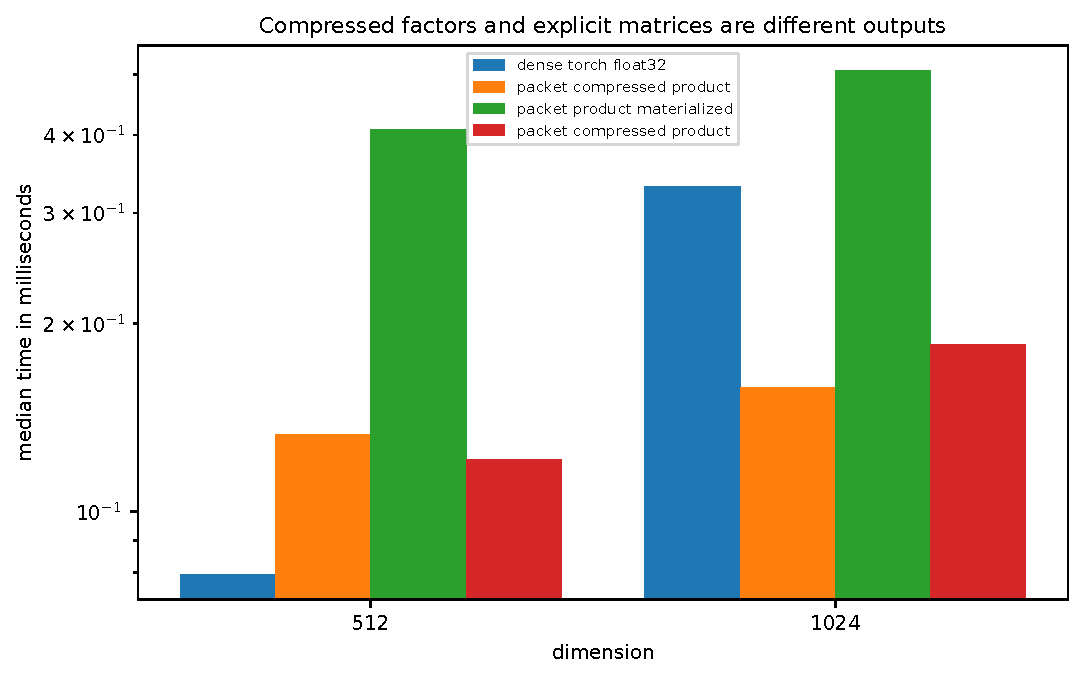
\includegraphics[width=.82\textwidth]{17_output_contract_timings.pdf}
\caption{Compressed and explicit products answer different computational questions.}
\label{fig:output_contracts}
\end{figure}

The algebra in \cref{thm:bdlr_product} explains why the compressed product can remain small. The materialization cost in \cref{prop:materialization_cost} explains why explicit output can erase the advantage.

\subsection{Discovery and transfer}

For hidden permuted blocks at dimension \(512\), structure discovery took \(2.1102\) ms, dense application took \(0.0969\) ms, and packet application took \(0.0151\) ms. The exact threshold in \cref{thm:amortization} is \(26\) uses. At dimension \(1024\), the corresponding values were \(5.2726\), \(0.1896\), and \(0.0241\) ms, giving \(32\) uses.

\begin{figure}[t]
\centering
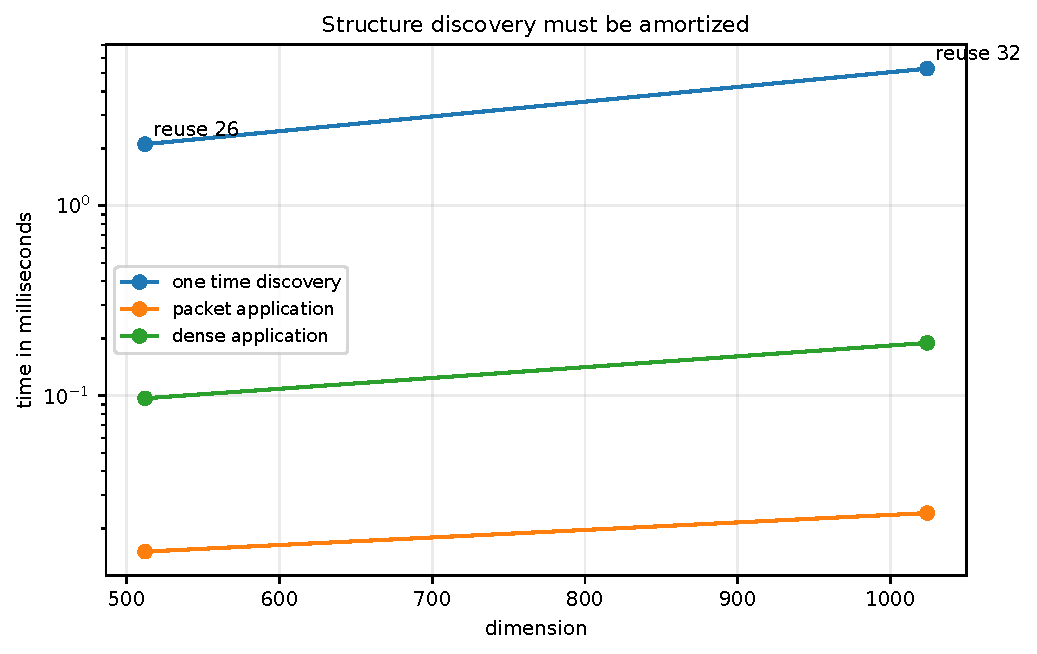
\includegraphics[width=.75\textwidth]{18_discovery_amortization.pdf}
\caption{A profitable repeated representation can remain unprofitable for one use.}
\label{fig:discovery}
\end{figure}

For one \(2048\) dense FP32 product, device resident graph replay took \(1.9993\) ms. The end to end pageable path took \(7.3036\) ms. The pinned path took \(6.3084\) ms. Two serial device resident products took \(3.6557\) ms, while the tested two stream path took \(4.2368\) ms.

\begin{figure}[t]
\centering
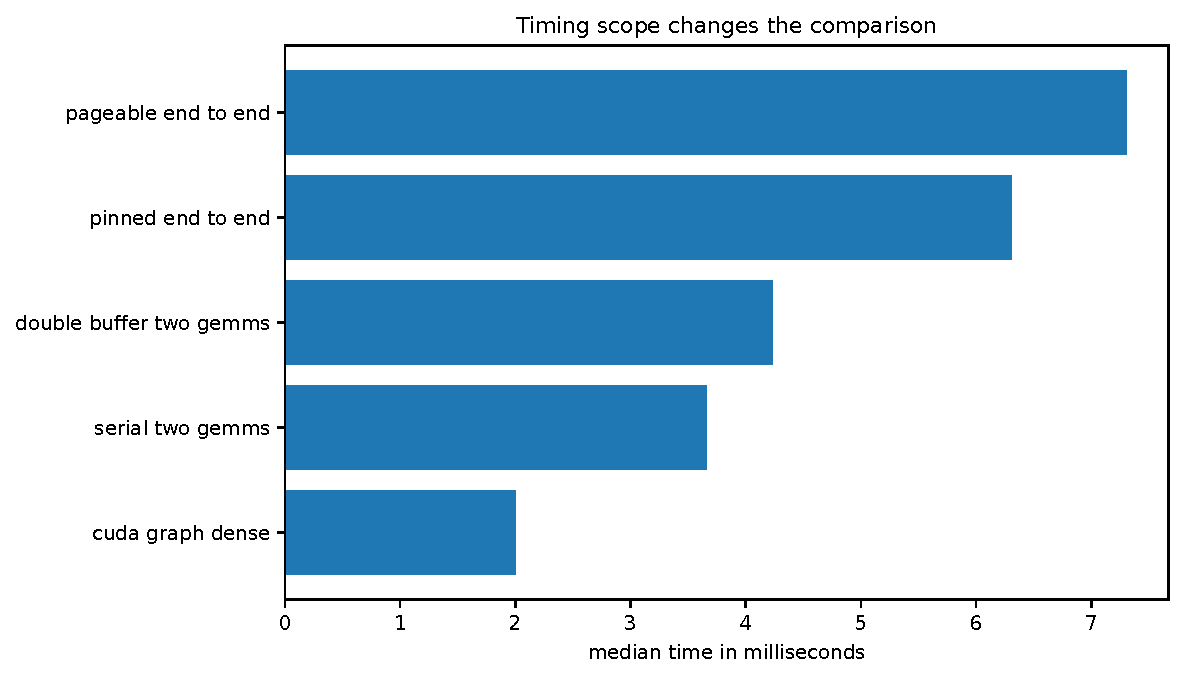
\includegraphics[width=.78\textwidth]{19_transfer_pipeline.pdf}
\caption{Device residence, transfer, graph replay, and a multioutput pipeline have different timing scopes.}
\label{fig:transfer_pipeline}
\end{figure}

\subsection{Negative controls}

The corpus retains methods that lost to their matched baselines.

\begin{itemize}
\item At dimension \(512\), recursive Strassen multiplication with leaf size \(128\) took \(7.0950\) ms, while the matched OpenBLAS dense multiplication took \(1.9597\) ms.
\item At dimension \(2048\), the tested recursive HODLR GPU path took \(5.6079\) ms, while dense GPU multiplication took \(0.0860\) ms.
\item The tested FP32 iterative refinement solve took \(22.0848\) ms, while the direct FP64 GPU solve took \(12.6286\) ms with a comparable final error.
\item The two stream dense path was slower than the serial two product path.
\item The GPU Walsh Hadamard transform was slower than the CPU implementation at length \(65536\), then became faster at length \(262144\).
\end{itemize}

Fast multiplication can be asymptotically valuable and still lose at measured sizes because of recursion, memory traffic, and kernel granularity. Hierarchical matrix methods have similar crossover issues \cite{AmbikasaranDarve2013}. Transform algorithms and tensor factorizations form additional structure classes \cite{CooleyTukey1965,Oseledets2011}.

\begin{figure}[t]
\centering
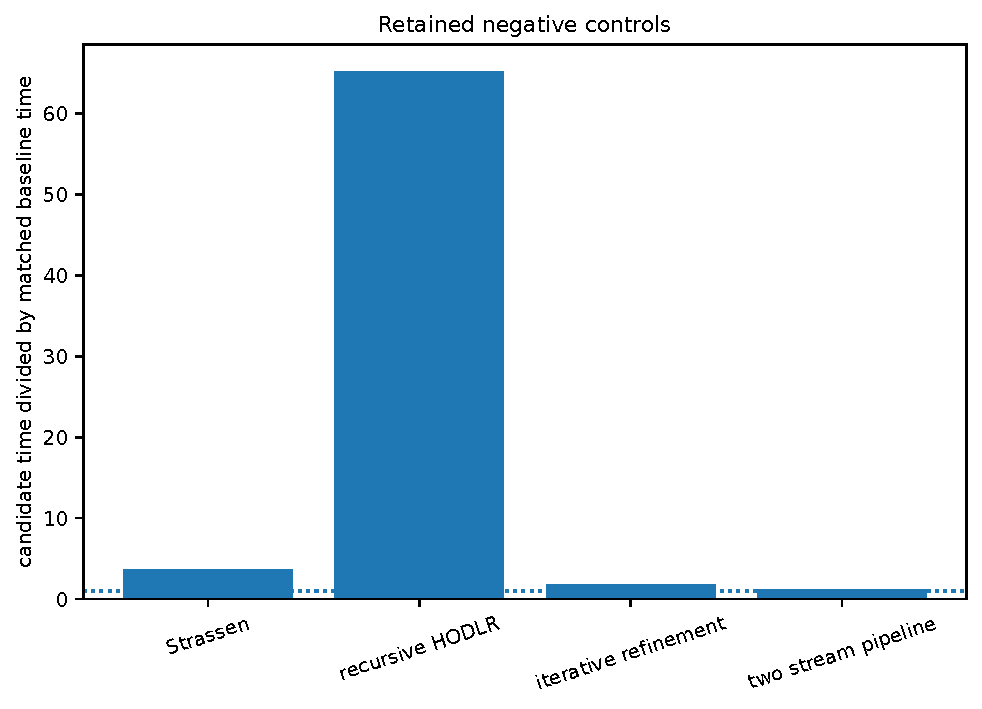
\includegraphics[width=.77\textwidth]{20_negative_controls.pdf}
\caption{Values above one are slowdowns against the matched baseline.}
\label{fig:negative_controls}
\end{figure}

\begin{figure}[t]
\centering
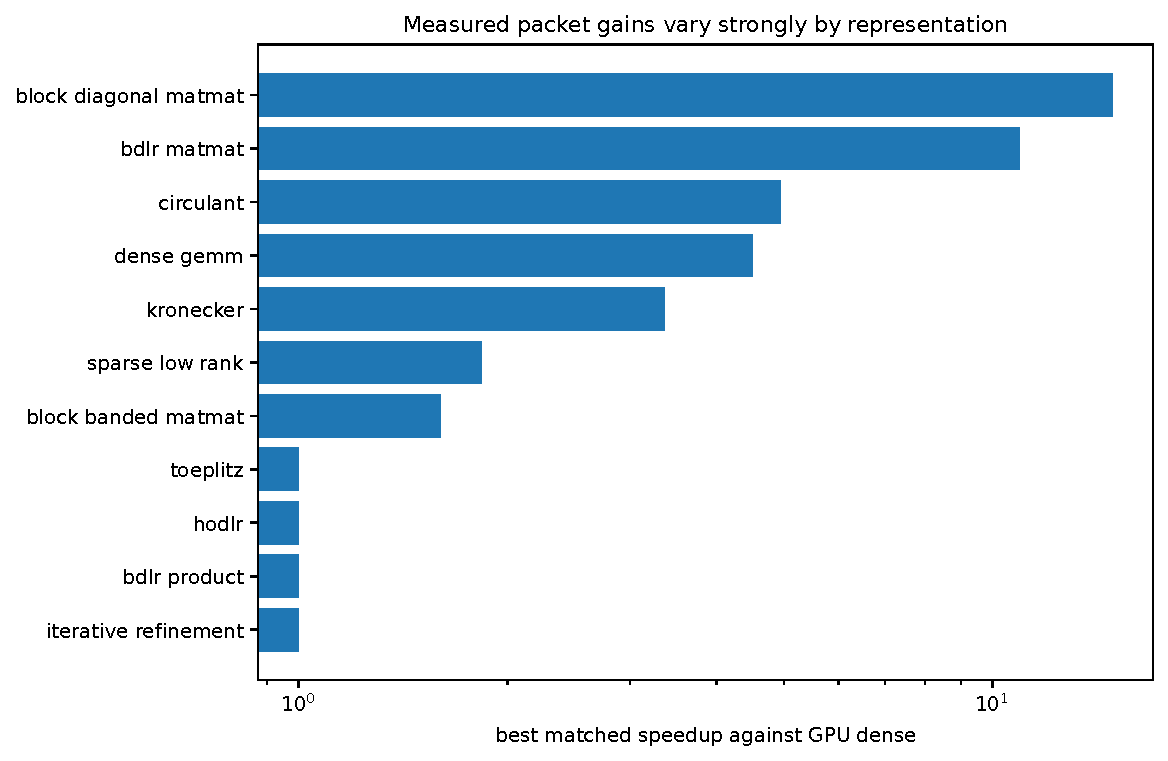
\includegraphics[width=.78\textwidth]{21_best_gpu_speedups.pdf}
\caption{The best matched gain differs strongly across suites. Regular packet structure dominates the largest measured rows.}
\label{fig:best_speedups}
\end{figure}

\section{Implementation and verification}\label{sec:implementation}

The release contains a small reference implementation of the exact operators and optimization algorithms used in the paper. The mathematical interface is deliberately narrow.

\begin{enumerate}
\item A packet layout records dimensions and coordinate slices.
\item A packet operator stores active blocks and evaluates them without materializing inactive blocks.
\item BDLR factors support exact application, product, solve, and small core recompression.
\item Graph utilities compute support products, path closure, Schur fill inclusion, and topological levels.
\item Tree dynamic programs solve the Lagrangian and quantized budget models.
\item A multiple choice dynamic program assigns discrete precision options.
\item Benchmark utilities audit case identity, output contracts, timing scopes, and retained negative controls.
\end{enumerate}

The full deterministic verifier performs \(37392\) checks in nine groups. It covers packet evaluation, adjoints, composition, structured primitives, recompression optimality, product chain error, graph support, Schur fill, tree compilation, precision assignment, and the benchmark corpus. The strengthened unit suite contains eleven passing tests. The original source suite contains twenty three passing tests for BDLR operations, Krylov methods, mixed precision, measured data schema, and figure generation.

\begin{table}[t]
\centering
\small
\begin{tabular}{>{\raggedright\arraybackslash}p{.34\textwidth}>{\raggedright\arraybackslash}p{.55\textwidth}}
\toprule
Layer & Verification target \\
\midrule
Packet semantics & materialization, application, adjoint, composition \\
Low rank algebra & exact product, Woodbury solve, optimal core recompression \\
Graph algorithms & path support, topological levels, Schur fill inclusion \\
Optimization & Lagrangian tree compiler, budget compiler, precision assignment \\
Numerical bounds & product chain error, block perturbation, clipped allocation \\
Empirical corpus & row count, suite count, device split, status, error ceiling \\
Document & proofs, labels, citations, figures, font embedding, render audit \\
\bottomrule
\end{tabular}
\caption{Verification layers in the strengthened release.}
\label{tab:verification_layers}
\end{table}

\section{Hardware implications and exact boundaries}\label{sec:boundaries}

The finite results suggest a device interface with grouped block kernels, low rank contractions, packet metadata, a transfer graph scheduler, and per edge precision tags. Such an interface may reduce materialization and repeated launch work when the operator family remains closed under the chosen representation.

The exact results stop at a finite candidate tree and a declared device model. Three broader problems remain open.

\begin{enumerate}
\item A universal discovery algorithm would need to find a profitable packet structure from an arbitrary operator and data distribution. The simultaneous spectral theorem and randomized low rank approximation cover special cases only.
\item A universal compiler would need a controlled approximation factor when costs are nonlocal and candidate decompositions overlap. The dynamic programs in \cref{thm:tree_compiler,thm:budget_compiler} do not cover that setting.
\item A packet native memory hierarchy would need a communication theorem for a family of operators and a specified architecture. The one pass byte model in \cref{prop:streaming_bytes} is not such a lower bound.
\end{enumerate}

Communication lower bounds require explicit machine models \cite{HongKung1981,BallardDemmelHoltzSchwartz2011}. CUDA Graph behavior and kernel constraints depend on the installed CUDA platform \cite{NVIDIA2026}. The measured results in this paper do not prove an optimal accelerator.

The article also makes no claim about the exponent of generic dense matrix multiplication. Packet algorithms answer a different question. They exploit a restricted operator class and may return a compressed output.

\section{Conclusion}\label{sec:conclusion}

A packet operator representation records which block maps exist, how they are stored, and what output they denote. Exact block evaluation and composition turn the support graph into algebra. Arithmetic, storage, and one pass data movement follow from the active block dimensions. Block diagonal plus low rank operators remain closed under multiplication before recompression. Their inverse is reduced by Woodbury, and their correction can be recompressed optimally through a small singular value problem.

Sparse transfer graphs predict path support, triangular schedule depth, and possible fill under elimination. Packet diagonal structure gives local Krylov spaces and a certified block Jacobi condition bound. Packetwise perturbations give a direct mixed precision certificate. Continuous tolerances follow from a convex allocation, while finite data type choices lead to an exact multiple choice budget program.

A finite candidate refinement tree supports a genuine packet compiler. The Lagrangian optimum, the quantized error budget optimum, and local recompilation are exact under additive hypotheses. This is narrower than unrestricted automatic discovery, but it turns one broad compiler conjecture into a proved algorithmic statement.

The measured corpus shows the practical distinction between regular and irregular structure. Equal block and BDLR operators gained substantially on the recorded GPU. Recursive HODLR, Strassen, iterative refinement, a small transform, and an attempted overlap lost to matched baselines. Discovery, transfer, capture, and materialization changed the break even point.

The computational principle is therefore precise. Remove work through a verified representation. Preserve the declared output. Compile only inside a model whose costs and errors are stated. Assign precision by sensitivity. Amortize one time costs. Keep negative controls. Treat the final timing as a property of the representation, device, kernel, and reuse regime together.

\section*{Language model contribution}

An OpenAI language model was used to help reorganize the original manuscript, test alternative theorem formulations, draft portions of the exposition, and design finite verification calculations. Its mathematical suggestions affected the packet intermediate representation, the small core recompression theorem, the product chain error bound, the quantized precision program, the exact tree compiler, the local recompilation theorem, and the separation of benchmark contracts. The author is responsible for checking every statement, proof, citation, computation, and measured claim in any submitted version. The model is not an author.

\bibliographystyle{amsplain}
\bibliography{PSC_Paper_VIII_Strengthened_Annals_Edition}

\end{document}
